\documentclass{report}
\usepackage{hyperref}
\usepackage[ngerman]{babel}
\usepackage{amsmath}
\usepackage{amsfonts}
\usepackage{amsthm}
\usepackage{tcolorbox}
\usepackage[a4paper, total={7in, 9in}]{geometry}
\usepackage[font={scriptsize,it}]{caption}
\usepackage{scrextend}
\usepackage{graphicx}
\usepackage{caption}
\usepackage{subcaption}
\usepackage[utf8]{inputenc}
\usepackage[T1]{fontenc}
\DeclareUnicodeCharacter{2212}{-}
\usepackage{verbatim}
\usepackage{tikz}

\tikzset{
  treenode/.style = {shape=rectangle, rounded corners,
                     draw, align=center,
                     top color=white, bottom color=blue!20},
  root/.style     = {treenode, font=\Large, bottom color=red!30},
  env/.style      = {treenode, font=\ttfamily\normalsize},
  dummy/.style    = {circle,draw}
}

\tikzstyle{level 1}=[level distance=3.5cm, sibling distance=3.5cm]
\tikzstyle{level 2}=[level distance=3.5cm, sibling distance=2cm]

% floating figure for column
\newenvironment{Figure}
	{\par\medskip\noindent\minipage{\linewidth}}
	{\endminipage\par\medskip}

\theoremstyle{definition}
\newtheorem{definition}{Definition}

\theoremstyle{example}
\newtheorem*{example}{Example}

\begin{document}

\begin{titlepage}
   \vspace*{\stretch{1.0}}
   \begin{center}
      \Large\textbf{BSY - FS20}\\
      \large\textit{Pascal Brunner - brunnpa7}
   \end{center}
   \vspace*{\stretch{2.0}}
\end{titlepage}


\tableofcontents
\newpage

\chapter{Vorlesung 1 - Übersicht und Geschichte der Betriebssyteme}

\section{Sie können den Begriff Betriebssystem erklären}
Das Betriebssystem soll die Komplexität mindern, also dem Programmierer einen Befehlssatz bereitstellen, der einfach zu beherrschen ist und interne Details vor dem Nutzer verbirgt.\\

\textbf{Aufgaben}\\
	\begin{itemize}
		\item Erweiterte (virtuelle) Maschine, die einfach zu programmieren ist
		\item Ressourcenmanager $\rightarrow$ verwaltet die vorhanden Hardware-Ressourcen (bspw. Speicher, CPU)
		\item Kontrollinstanz für jegliche Zugriffe
	\end{itemize}
	\\

\textbf{Bestandteile $\rightarrow$ Programme im Systemmodus (Kernel Mode)}
	\begin{itemize}
		\item Gerätetreiber
		\item Prozessmanager
		\item Fenstermanager
	\end{itemize}
	
\textbf{Systemaufrufe} sind Schnittstellen zwischen Anwendungsprogrammen und Betriebssystem

\section{Sie können die Begriffe Batchbetriebssystem, Uniprogramming, Multiprogramming, Time sharing erklären und diskutieren}
	\subsection{Batchsysteme}
		\begin{itemize}
			\item Anwender übergibt Job (Lochkarten oder Band) an den Operator
			\item Der Operator reiht mehrere Jobs sequentiell in einem Eingabegerät auf $\rightarrow$ Batch
			\item ein spezielles Programm, der Monitor kontrolliert Ausführung der Jobs im Batch
			\item Hilfsprogramme werden nach Bedarf eingelesen
		\end{itemize}
		
	\subsection{Uniprogramming}
		\begin{itemize}
			\item Es befindet sich nur ein Programm im Speicher.
			\item I/O Operationen sind sehr langsam im Vergleich zur Ausführung von Instruktionen $\rightarrow$ CPU oft idle
			\item Programme mit viel I/O Operationen haben eine schlechte CPU Auslastung und verbringen die meiste Zeit mit warten		
		\end{itemize}

	\subsection{Multiprogramming}
		\begin{itemize}
			\item Mehrere Programme im Speicher, Programm wartet auf I/O Operation und der Monitor führ ein anderes Programm aus
			\item Multiprogramming / Multitasking
		\end{itemize}
		
		\textbf{Hardwareunterstützung}\\
		\begin{itemize}
			\item I/O Interrupts $\rightarrow$ Programmumschaltung möglich
			\item (wenn möglich) DMA
			\item Speicherverwaltung (Memory Management)
		\end{itemize}
		
		\textbf{Softwareunterstützung}\\
		\begin{itemize}
			\item Scheduling
			\item Steuerung und Kontrolle von Ressourcenzugriff
		\end{itemize}
		
	\subsection{Time Sharing Systeme (TSS)}
		\begin{itemize}
			\item Batch Multiprogramming $\rightarrow$ Keine Interaktion mit Anwender
			\item Erweiterung Multiprogramming $\rightarrow$ Concurrency; CPU-Zeit auf mehrere Benutzer verteilt;
		\end{itemize}
		\textbf{Wieso funktioniert das?}\\
		Der Mensch hat mit eine lange Reaktionszeit, diese Zeit wird verwendet damit andere User das System brauchen können. Dies benötigt ca. 2 Sekunden Rechenzeit pro Minute $\rightarrow$ ca. 30 Anwender könnten ohne wahrnehmbare Verlängerung der Reaktionszeit ($\leq$100ms) das System gemeinsam nutzen.

	\section{Sie können den Begriff Monitor erklären}
Der Monitor gilt als ein Minimalsystem, welches bei der Initialisierung die nicht gebrauchten Vektoren auf den Default Wert setzen. Es bietet einfache Schnittstellen, so dass die HW nicht beschädigt wird.  Des Weiteren hat es eine einfache Kommunikation mit dem Anwender:
\begin{itemize}
	\item setzen und lesen von Parametern, Speicher, etc.
	\item laden von Programmen
	\item debuggen von Programmen
\end{itemize}
\\
Bei komplexere Systemen (bspw. BIOS) werden noch weitere HW-Komponenten (Cache Controller oder Memory Management Unit) geladen; der Speicher wird auf die korrekte Funktionalität geprüft.\\
\textbf{Batch-Systeme: Monitor}
\begin{itemize}
	\item Monitor liest Job um Job vom Eingabegerät
	\item Monitor legt Job im Anwendungsprogramm-Bereich ab
\end{itemize}

\section{Sie können Problemstellungen bei frühen Betriebssytemen aufzählen}
	\begin{itemize}
		\item Probleme mit nicht deterministischem Programmverhalten $\rightarrow$ Resultat der Berechnung abhängig von anderen aktiven Programmen
		\item Probleme mit gegenseitigem Ausschluss $\rightarrow$ mehr als ein Programm greift gleichzeitig auf Ressource zu
		\item Probleme mit der Synchronisation $\rightarrow$ Signale beim Warten verloren
		\item Probleme mit Deadlocks $\rightarrow$ Programme warten gegenseitig bspw. Freigabe
	\end{itemize}

\section{Sie können die grundlegende Konzepte von Betriebssystemen aufzählen und diskutieren}
	\begin{enumerate}
		\item Prozesse
		\begin{itemize}
			\item Programm in Ausführung $\rightarrow$ Sandbox
		\end{itemize}
		\item Scheduling und Ressourcenverwaltung
		\begin{itemize}
			\item Zuteilung von Rechenleistung
			\item BS unterhält Queueus (Ready, Wait, Long Term Queue)
		\end{itemize}
		\item Datenmanagement (Speicherverwaltung, File-Systeme)
		\item Schutz und Sicherheit
		\item System-Architektur
	\end{enumerate}

\section{Sie können die aktuelle Betriebssystemtypen aufzählen, erklären und diskutieren}
\textbf{TBD}

\section{Sie können die Begriffe Multithreading und symmetrisches Multiprocessing erklären und diskutieren}
\textbf{TBD}



\chapter{Vorlesung 2 - Computer Systeme}

\section{Sie können für das Betriebssysteme wichtige Rechnerkomponenten aufzählen und erklären}
	\begin{itemize}
		\item {Prozessor (CPU)\\
		Heute oft mehrere CPU's pro Prozessor, wobei man diese dann in unterschiedliche Threads aufteilt. Pro Core hat man dann eine ALU, dementsprechend verwenden die Threads dann die ALU zusammen. Die Grundidee dabei ist, dass man möglichst gut parallelisieren kann $\rightarrow$ wobei die Optimierung pro Core nicht linear ansteigt.}
		\item {Hauptspeicher $\rightarrow$ Daten und Code\\
		Diese Aufteilung kann man dann unterschiedlich aufteilen, wie man die Memory teilen möchte.
\begin{itemize}
	\item Uniform Memory Access (UMA) $\rightarrow$ alle Speicherzugriffe gleich lang
	\item Non-Uniform Memory Access (NUMA) $\rightarrow$ ein Adressraum, der Speicher ist jedoch langsamer. Des Weiteren muss das Memory Management berücksichtigt werden
\end{itemize}}		
		\item I/O Module $\rightarrow$ Sekundärspeicher, Tastatur, Bildschirm etc.
		\item Bus $\rightarrow$ verbindet CPU - Speicher - I/O
	\end{itemize}

\section{Sie können Aufgaben und Funktionsweise der CPU aufzählen und erklären}
\textbf{Recheneinheiten}\\
\begin{itemize}
\item ALU (Arithmetic and Logic Unit $\rightarrow$ Integer- und Bitoperationen)
\item FPU (Floating Point Unit)
\end{itemize}

\textbf{Adress-, Daten und Statusregister (PSW)}\\
 \begin{itemize}
 	\item für Benutzer sichtbar
 	\item von System- und Anwenderprogramme benutzt
 \end{itemize}
 
\textbf{Kontroll- und Steuerregister}\\
\begin{itemize}
	\item viele nicht sichtbar
	\item z.T. von CPU genutzt
\end{itemize}

\textbf{Instruction (Control) Unit}\\
\begin{itemize}
	\item Steuereinheit
\end{itemize}

\textbf{Bus Interface Unit}\\
\begin{itemize}
	\item Ansteuerung der externen Einheiten
\end{itemize}

\textit{EVTL: Bild einfügen}

\textbf{Programmier-Model}\\
\begin{itemize}
	\item Beim Programmieren muss man sich mit den \textit{CPU Registern} (Daten, Stack, PC) auseinandersetzen. 
	\item Der \textit{Instruktionssatz} kann sich je nach Chipmodel anpassen
	\item \textit{Memory} ist ein linearer Addressraum, die Addressierung erfolgt in Bytes und Worte. Die kleinste Einheit ist ein Byte
	\item \textit{I/O-Geräte} $\rightarrow$ memory mapped I/O (var1) oder dedicated I/O (var2). Diese Module dienen Daten vom und zum System-Bus zu liefern. Diese 
\end{itemize}
		

\section{Sie können Interrupts im Zusammenhang mit Betriebssystemen erklären und diskutieren}
Im Wesentlichen nutzt man Interrupts um hin- und her zu schalten. Es unterbricht die aktuelle Ausführung eines Prozesses.

\textit{asynchrone Interrupts}:
\begin{itemize}
	\item Timer $\rightarrow$ Aus Sicht des Programmes planbar
	\item I/O Devices $\rightarrow$ Aus Sicht des Programmes nicht vorhersehbar
	\item Hardwarefehler $\rightarrow$ Aus Sicht des Programmes nicht vorhersehbar
\end{itemize}

\textit{synchrone Interrupts}:
\begin{itemize}
	\item Program $\rightarrow$ bspw. div durch 0
	\item Trap, SWI
\end{itemize}

Die Kontrolle über diese Interrupts, wird durch den sogenannten Interrupt Handler (ISR) - $\rightarrow$ als Vektor-Tabelle dargestellt - dargestellt und kontrolliert. Wobei nur das Betriebssystem, die Vektortabelle setzen kann.

\section{Sie können Kernel und User Mode erklären und diskutieren}
Die meisten Prozessoren arbeiten in zwei Modi\\

\begin{itemize}
	\item Kernel Mode
	\item User Mode
\end{itemize}

\textbf{Kernel Mode}\\
Ist ein priviligierte Mode $\rightarrow$ unbeschränkter Zugriff auf alle Instruktionen und Ressourcen.\\
Drei Wege um vom User Mode zum Kernel Mode zu wechseln
\begin{itemize}
	\item Syscall
	\item Interrupt
	\item Exception
\end{itemize}

\textbf{User Mode / System Mode}\\
Ist ein nicht priviligierter Mode mit beschränktem Zugang zu kritischen Instruktionen, kein Zugang zu System Timer, Interrupt Controller oder System Control Block. Des Weiteren besteht ein beschränkter Zugriff auf Speicher Peripherie.
\begin{itemize}
	\item beschränkter Zugriff $\rightarrow$ 'Sicherer Modus'
\end{itemize}


\section{Sie können die Funktionsweise von System Calls erklären}
Grundsätzlich geht es darum eine Schnittstelle zwischen Anwendersoftware und Systemsoftware zu erstellen. Es schaltet zwischen Kernel und User Mode um.\\
\textbf{Ablauf}\\
\begin{enumerate}
	\item Anwenderprogramm stellt Parameter bereit (Register, Stack)
	\item ruft Bibliotheksfunktion auf $\rightarrow$ normaler Prozeduraufruf (oft Assembler Programm und setzt System Call Number)
	\item Syscall bzw. SWI $\rightarrow$ Kontrolle geht an Kernel $\Rightarrow$ priviligierter Modus (wobei der Kernel den System Call Handler aufruft und der Handler ausgeführt wird)
	\item evtl. Rückkehr zur Bibliothektsfunktion $\rightarrow$ Kann zu anderen Anwenderprogramme umschalten (falls System Call blockiert oder ein anderes Anwenderprogramm Rechenzeit benötigt.)
	\item Rückkehrs ins Anwenderprogramm
\end{enumerate}

\textbf{TBD - Codebeispiel Vorlesung 2 Seite 17 einfügen}

\section{Sie können I/O Module und -Kommunikation beschreiben und diskutieren}
Es wird zwischen drei Techniken der Kommunikation unterschieden:\\
\textbf{Programmed I/O oder synchroner I/O}:\\
\begin{itemize}
	\item benötigt keine Interrupts
	\item CPU wartet auf Beendigung jeder einzelnen I/O Operationen
	\item Unschönheit: busy wait $\rightarrow$ die CPU wartet bis alles beendet wurde $\Rightarrow$ der Zeitfaktor ist hier bei ca. $10^6$
\end{itemize}

\textbf{Interrupt Driven I/O oder asynchroner I/O}:\\
\begin{itemize}
	\item CPU führt während I/O Operation Code aus
	\item Wird unterbrochen, wenn I/O Operation beendet
	\item Die CPU kann andere Arbeiten ausführen, bis das Vorherige beendet wurde
\end{itemize}

\textbf{Direct Memory Access (kurz: DMA}:\\
\begin{itemize}
	\item Man schaltet die CPU direkt mit dem Memory
	\item Ein Speicherblock mit Daten wird vom/zum Speicher übertragen
	\item ohne Rechenleistung der CPU zu beanspruchen
	\item gibt einen Interrupt, wenn Transfer beendet
	\item CPU nur zu Beginn und zu Ende des Transfer benötigt
	\item CPU kann dazwischen andere Arbeiten ausführen
\end{itemize}

\section{Sie können die Speicherhierarchie moderner Prozessorsysteme erklären und diskutieren und die mittlere Zugriffszeit berechnen}
Zwischen Register und Hauptspeicher liegt ein Verhältnis von x100.\\


Zwischen Hauptspeicher und Disk liegt ein Verhältnis von x1'000'000 - im Vergleich ist dies 1s zu 12 Tagen. \\

Aus diesem Grund lohnt es sich ein entsprechendes Konzept aufzubereiten, damit man die häufigen Daten schnell zur Verfügung hat. Dabei unterscheidet man vor allem zwischen Cache Level 1 - 3
\begin{Figure}
\centering
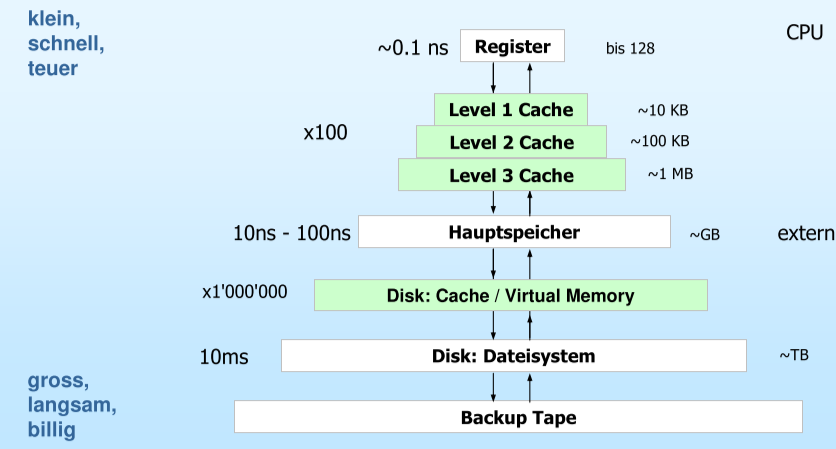
\includegraphics[width=500px]{img/Speicherhierarchie.png}
	\captionof{figure}{Abbildung der Speicherhierarchie}
	\label{fig:Speicherhierarchie}
\end{Figure}

	\subsection{Cache}
Beim Cache möchte man die wichtigen Daten möglichst nahe an der CPU halten. So dass man möglichst wenig Block Transfers zwischen Cache und Main Memory. Befindet sich das ein Wort im Wort, dann kann man dies direkt an die CPU übermitteln. Ist das Wort nicht im Cache, so muss man den kompletten Memory Blcok laden, in welchem sich das Wort behandelt.\\
Das ganze ist transparent für den Benutzer, dies bedeutet, dass er dies (abgesehen von der Ladezeit) nicht wirklich merkt.\\

		\subsubsection{Wieso funktioniert das? $\rightarrow$ Lokalitätsprinzip}
Dies funktioniert aufgrund des Lokalitätsprinzip. Man unterscheidet zwischen räumliche Lokalität und zeitliche Lokalität. \\
\begin{itemize}
	\item räumliche Lokalität (spacial locality) $\rightarrow$ grosse Wsk, dass nächster Speicherzugriff, nahe liegende Daten stattfindet (Bspw. Array-Zugriff)
	\item zeitliche Lokalität (temporal locality) $\rightarrow$ grosse Wsk, dass Speicherzugriff auf gleiche Daten nochmals stattfindet (Bspw. for-Schleife)
\end{itemize}

		\subsubsection{Wie funktioniert es?}
\textbf{Hitrate (hit ratio)}: h\\
\textit{h}: Wahrscheinlichkeit, dass der Speicherzugriff die Daten im Cache findet\\

\textit{m}: Missrate (miss ratio): $m=1-h$\\

\textbf{Mittlere Zugriffszeit $t_a$}\\
\begin{itemize}
	\item Zugriffszeit auf nächsten Speicher $T_N$ gegeben
	\item hit ratio h gegeben
	\item einstufiger Cache gegeben
\end{itemize}

\begin{equation}
\begin{split}
	T_a &= T_C + (1-h) * T_N\\
	T_a &= T_C + m * T_N
\end{split}
\end{equation}

\begin{Figure}
\centering
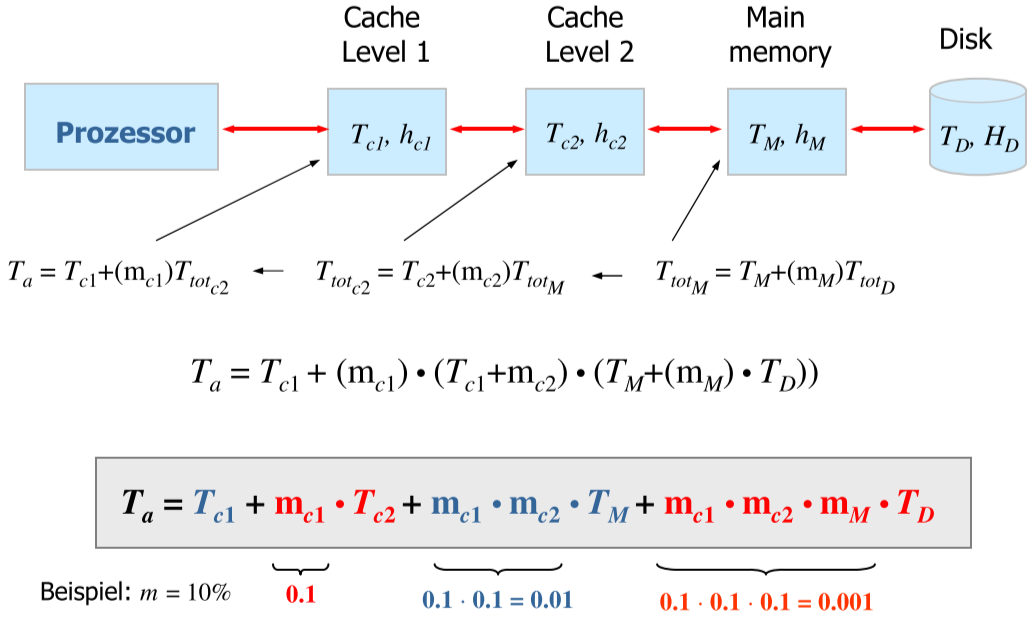
\includegraphics[width=500px]{img/BerechnungCacheLevel.png}
	\captionof{figure}{Berechnung der verschiedenen Cache Level 1-3}
	\label{fig:Speicherhierarchie}
\end{Figure}

\section{Sie können den Startvorgang einer Betriebssystems erklären}
Das Betriebssystem startet in zwei wesentlichen Phasen\\
\begin{itemize}
	\item hardwareabhängige Phase
	\item Start der eigentlichen Betriebssystems
\end{itemize}

\textbf{Hardwareabhängige Phase}:\\
\begin{itemize}
	\item Prozessor startet auf seiner Reset-Adresse
	\item Code aus Festwertspeicher (ROM, Flash) auf Platine ausgeführt $\rightarrow$ Hardwareüberprüfung, initialisiert Minimalzugriff auf Disk oder Netzwerk
\end{itemize}

\textbf{Betriebsabhängige Phase}:\\
\begin{itemize}
	\item Boot Code wird ausgeführt $\rightarrow$ steuert alle weiteren Schritte
\end{itemize}

\begin{enumerate}
	\item Der Prozessor startet das BIOS (Basic Input Output System(
	\item BIOS testet das System (POST) und lädt Master Boot Record (MBR) vom ersten Sektor des ersten Disks
	\item Der MBR-Code liest den Boot-Code von der ersten aktiven Partition und startet den Boot-Code (Loader)
	\item der Boot-Code lädt sich weitere Informationen (Files) zum Startet des Betriebssystems von der Partition
\end{enumerate}


\chapter{Vorlesung 3 - Prozesse und Threads}

\section{Sie können den Begriff Prozess erklären}
\begin{itemize}
	\item Ein Prozess ist eine Instanz eines Programmes in Ausführung
	\item Man schafft pro Prozess einen Kontext $\rightarrow$ Prozessenthält Kontextinformationen
	\item Prozess muss nicht zwingend aktiv sein $\rightarrow$ einer der wichtigen Fragestellungen, wie viele Prozesse darf ich gleichzeitig laufen lassen?
	\item Dadurch entsteht eine Kapselung $\rightarrow$ Sandbox-Konzept
\end{itemize}

\begin{Figure}
\centering
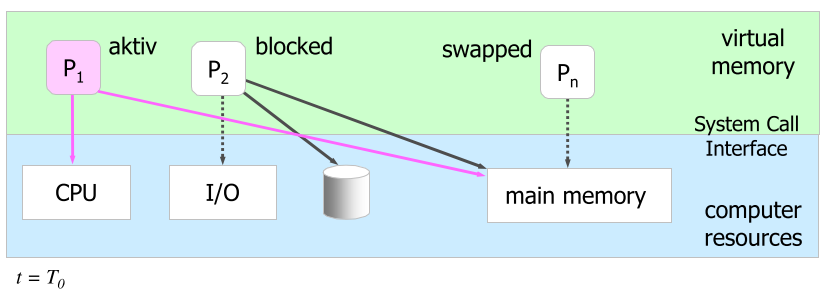
\includegraphics[width=500px]{img/SchnappschussLaufzeit.png}
	\captionof{figure}{Schnappschus seiner Laufzeitumgebung im Prozess-Kontext}
	\label{fig:Schnappschuss Prozess Kontext}
\end{Figure}

\textbf{Zwei Sichtweise}\\
\begin{itemize}
	\item \textbf{Unit of Resource Ownership} $\Rightarrow$ Eine Einheit, die Ressourcen besitzt; ein virtueller Adressraum, in dem das Prozess Image steht; Kontrolle über Ressourcen
	\item \textbf{Unit of Scheduling} $\Rightarrow$ Eine Einheit, die schedulierbar ist; CPU-Scheduler weist der CPU einen Prozess zu (dispatch); zum Prozess gehören der Executino State (PC, SP, Register) und Ausführungspriorität
\end{itemize}
\section{Sie können erklären, wie Prozesse auf einer CPU ausgeführt werden}
\begin{itemize}
	\item Prozesse werden gleichzeitig (concurrent) ausgeführt. Ihre Ausüfhrung wird auf einer CPU verschränkt
	\item Prozesse können in der Ausführung unterbrochen und später weiterverarbeitet werden
\end{itemize}

\begin{Figure}
\centering
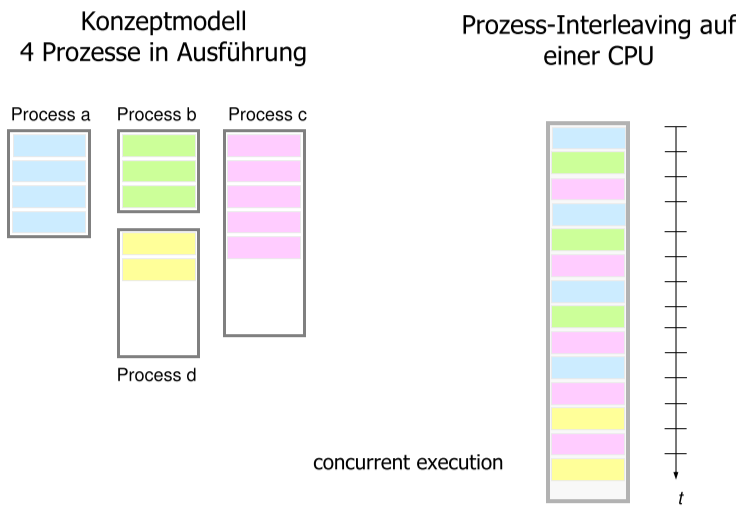
\includegraphics[width=500px]{img/Prozessausfuehrung.png}
	\captionof{figure}{Prozessausführung einer CPU}
	\label{fig:Prozessausführung einer CPU}
\end{Figure}

\section{Sie können die Beschreibung der Prozessausführung erklären und skizzieren}
	\subsection{zeitliches Verhalten}
\begin{itemize}
	\item Zustandsmodell
	\item Beschreibt den aktuellen Zustand eines Prozesses, z.B. Running oder Not-Running
\end{itemize}

\begin{Figure}
\centering
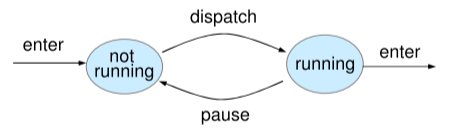
\includegraphics[width=500px]{img/ProzessausfuehrungZeitlich.png}
	\captionof{figure}{Prozessausführung einer CPU zeitliches Verhalten}
	\label{fig:Prozessausführung einer CPU zeitliches Verhalten}
\end{Figure}

$\Rightarrow$ In der Realität sieht dieses Zustandsdiagram wesentlich komplexer aus:\\
\begin{Figure}
\centering
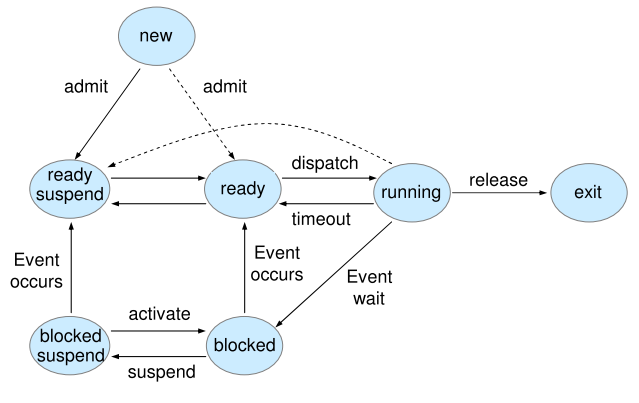
\includegraphics[width=500px]{img/ProzessausfuehrungZeitlichReal.png}
	\captionof{figure}{Prozessausführung einer CPU zeitliches Verhalten (Realität)}
	\label{fig:Prozessausführung einer CPU zeitliches Verhalten (Realität)}
\end{Figure}

	\subsection{örtliches Verhalten}
\begin{itemize}
	\item Queuing-Diagram
	\item Beschreibt den Ort, wo sich Prozesse aufhalten, wenn Sie sich in einem bestimmten Zustand befinden
	\item Mehrere Prozesse können im gleichen Zustand befinden, z.B. Not-Running, in diesem Fall warten sie in einer Warteschlange
\end{itemize}	
	
\begin{Figure}
\centering
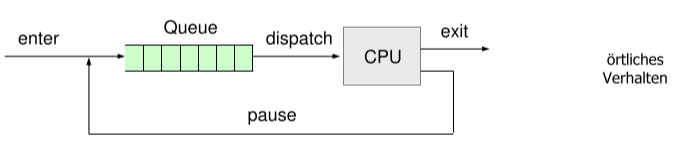
\includegraphics[width=500px]{img/ProzessausfuehrungOertlich.png}
	\captionof{figure}{Prozessausführung Örtliches Verhalten}
	\label{fig:Prozessausführung einer CPU örtliches Verhalten}
\end{Figure}

$\Rightarrow$ In der Realität sieht diese Queue wesentlich komplexer aus:\\
\begin{Figure}
\centering
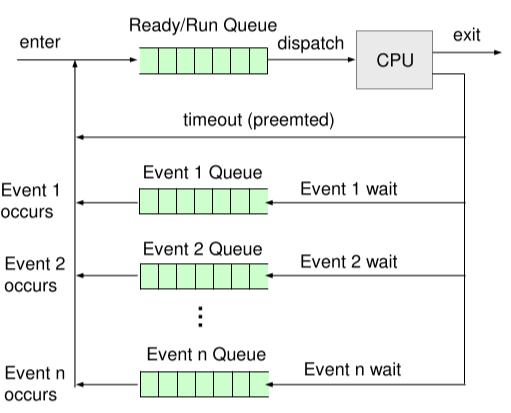
\includegraphics[width=500px]{img/ProzessausfuehrungOertlichReal.png}
	\captionof{figure}{Prozessausführung Örtliches Verhalten (Realität)}
	\label{fig:Prozessausführung einer CPU örtliches Verhalten (Realität)}
\end{Figure}

\section{Sie können den Prozesswechsel und die Ausführungsmodi erklären}
Gründe für Prozesswechsel:\\
\begin{itemize}
	\item Timer (clock) $\rightarrow$ Zeitintervall abgelaufen $\Rightarrow$ Prozess geht in Zustand ready
	\item I/O Interrupt $\rightarrow$ auf Interrupt wartenden Prozess in den Zustand READY oder READY SUSPEND versetzen (Entscheid ob laufender Prozess unterbrochen wird oder nicht)
	\item Page fault (virtual memory)
	\item \textbf{TBD V03 - S.12}
\end{itemize}

Zwei Möglichkeiten für den Prozesswechsel:\\
\begin{enumerate}
	\item \textbf{Mode Switch}: Kein Prozesswechsel, nur Unterbruch $\rightarrow$ kostet nicht so viel Zeit
	\item \textbf{Context Switch}: Prozesswechsel, impliziert auch Mode Switch
\end{enumerate}

	\subsection{Prozessausführung Modi}
\begin{itemize}
	\item \textbf{User Mode}: weniger priviligiert $\rightarrow$ Anwenderprogramme\\
	\item \textbf{System Mode}: Mehr priviligiert $\rightarrow$ Betriebssystemfunktion
\end{itemize}

\section{Sie können erklären, wie Prozesse durch das BS verwaltet werden}
Das Betriebssystem unterhält und verwaltet verschiedenste Tabellen für die Verwaltung von Prozessen und Ressourcen.
\begin{itemize}
	\item Speicher $\rightarrow$ Memory Tabellen
	\item Geräte $\rightarrow$ I/O Tabellen
	\item Files $\rightarrow$ File Tabellen
	\item CPU $\rightarrow$ Prozess Tabellen
\end{itemize}
Die Informationen liegen in den verschiedenen Tabellen. Die oben erwähnten Tabellen werden konzeptionell von jedem Betriebssystem verwendet, jedoch unterscheidet sich dies in der Implementierung.\\
\textbf{wichtig}: Die Tabellen müssen selbst wieder miteinander verknüpft sein, d.h. ein Prozess muss wissen welche Files er benutzt etc.

		\subsubsection{Prozess Image}
Prozess Image
\begin{itemize}
	\item besteht aus Benutzerprogramm (code bzw. Text), Daten, Stack, Heap
	\item besteht Kontext im Prozesskontrollblock (PCB) gespeichert $\rightarrow$ PCB, eine Datenstruktur mit Zustandsinformationen zum Prozess
	\item sind im virtuellen Speicher abgelegt
\end{itemize}
Das Betriebssystem hat nur Zugriff auf Prozessdaten, wenn das Prozessimage teilweise im physikalischen Speicher steht.

		\subsubsection{Prozesskontrollblock PCB}
Das PCB ist eine der wichtigsten Datenstrukturen im Betriebssystem $\rightarrow$ es speichert Prozesskontext und ist Teil des Prozessimages. \\
Es enthält alle notwendigen Informationen zum Prozess:
\begin{itemize}
	\item Process Identification
	\item Process Control Information
	\item Process State Information
\end{itemize}

\section{Sie können die Prozesserzeugung am Beispiel Unix / Linux erklären und anwenden (Praktikum)}
nicht weiter relevant für mündlich Prüfung

\section{Sie können erklären und diskutieren, wie das Betriebssystem ausgeführt wird}


\chapter{Vorlesung 4 und 5 - Scheduling}

\section{Sie können den Begriff Scheduling erklären und diskutieren}

\section{Sie können die wichtigsten Scheduling Algorithmen aufzählen, erklären und diskutieren}

\section{Sie können die Scheduling Verfahren der wichtigsten Betriebssysteme erklären und diskutieren}

\section{Sie können Probleme beim Multiprozessor Scheduling aufzählen und erklären}
	\begin{itemize}
		\item Task läuft lange auf CPU $\rightarrow$ viele Daten ins Cache geladen $\Rightarrow$ beim CPU-Wechsel müssen die Daten neugeladen werden
		\item Task hält Spin-Lock $q$ läuft ab $\rightarrow$
	\end{itemize}
	
	\subsection{Space Sharing}
Verwandte Task bzw. mehrere Task (Threads) arbeiten zusammen. Scheduling mehrerer Tasks über mehrere CPU's.
\textbf{einfachstes Verfahren}:\\
\begin{itemize}
	\item non-preemptive $\rightarrow$ gestartet Tasks werden abgearbeitet
	\item CPU idle während Blocking
	\item Tasks nur starten wenn genügend CPU's verfügbar
	\item Vor-/Nachteilt $\rightarrow$ kein Overhead wegen Kontextwechsel und eher schlechtes Load-Balancing
\end{itemize}

\textbf{Alternatives Verfahren}:\\
\begin{itemize}
	\item zentrale Instanz (Server) überwacht Scheduling
	\item Anzahl Threads wird von Applikation dynamisch angepasst
\end{itemize}

	\subsection{Gang Scheduling}
\begin{itemize}
	\item man gruppiert verwandtre Threads gemeinsam zu einer \textit{Gang}
	\item Gang-Mitglieder sind gleichzeitig auf verschiedenen CPU's aktiv, welche gemeinsam starten und enden
\end{itemize}	

\section{Sie können den Begriff Real-Time Scheduling erklären und disktutieren}
\begin{itemize}
	\item Real-Time Ereignisse sind Systeme, welche auf die äussere Welt reagiert
	\item Ereignisse finden in der reellen Zeit statt $\rightarrow$ real-time
	\item intuitive Betrachungsweise $\rightarrow$ was bedeutet das System muss schnell reagieren?
\end{itemize}

Real-Time Systeme verhalten sich korrekt, wenn:
\begin{itemize}
	\item das logische Resultat einer Berechnung stimmt (Daten müssen beim Flugzeug real-time sein, beim Streaming ist es weniger schlimm)
	\item Das Resultat zum richtigen Zeitpunkt ausgeleifert wird (innerhalb der Deadline)
	\item Hard Real-Time Systeme $\Rightarrow$ Deadline \textbf{MUSS} eingehalten
	\item Soft Real-Time Systeme $\Rightarrow$ Deadline \textbf{Kann} eingehalten
\end{itemize}

	\subsection{Eigenschaften}
\begin{itemize}
	\item zeitkritische Task wiederholen sich in regelmässigen Abständen
	\item die Dauer und die benötigten Betriebsmittel sind bekannt
\end{itemize}

	\subsection{Drei Real-Time Task Klassen}
\begin{enumerate}
	\item kritische Tasks (periodische oder asynchrone bzw. sporadische Tasks)
	\item nicht kritische, aber notwendige Tasks
	\item nicht notwendige Tasks (nice to have)
\end{enumerate}


\section{Sie können die wichtigsten Real-Time Scheduling Algorithmen aufzählen, erklären und diskutieren}

	\subsection{Rate Monotonic Scheduling (preepmtive}
Statische Priorität eines Jobs proportional zu Repetitionsrate.\\
Das spannende dabei ist, dass die Grenze für erfolgreiches Scheduling berechnet werden kann \\
\textbf{Diskussion}:
\begin{itemize}
	\item eher konservativ, besserer Auslastung möglich
	\item Scheduling Algorithmus beliebig
	\item Grenzwert für n $\rightarrow$ $\inf$: $U_{tot} = ln * 2 \approx 0.69$
	\item konkrete Anwendungen: Auslastung bis 90 Prozent realistisch
\end{itemize}

	\subsection{Deadline Scheduling}
Tasks zum richtigen Zeitpunkt starten resp. beendet\\
\textbf{mögliche Deadlines}:
\begin{itemize}
	\item Start Deadline $\rightarrow$ Zeitpunkt zu dem ein Task gestartet werden muss
	\item Completion Deadline $\rightarrow$ Zeitpunkt an dem der Task beendet sein muss
\end{itemize}

\textbf{Earliest Deadline Scheduling}:
\begin{itemize}
	\item Priorität umgekehrt proportional zur Zeit bis Deadline
	\item Scheduling aufwendiger als bei RMS $\rightarrow$ Prioritäten müssen dynamisch angepasst werden
	\item Theoretische Auslastung bis zu 100 Prozent möglich
\end{itemize}

	\subsection{Cyclic Executives}
\begin{itemize}
	\item statisches Scheduling
	\item non-preemptive
	\item Schedule für periodischen Hauptzyklus (100ms) $\rightarrow$ mehrere Nebenzyklen
	\item Realisierung: Aufruf von Prozeduren
\end{itemize}

\chapter{Vorlesung 6 - Synchronisation}
Die Begrifflichkeiten \textit{Prozesse und Threads} werden hier als \textit{Tasks} zusammengefasst

\section{Sie können Problemstellungen um Nebenläufigkeit und Parallelverarbeitung aufzählen und diskutieren}
\begin{itemize}
	\item nebenläufige Tasks nutzen im Auftrag gemeinsam Daten und Ressourcen
	\item Nicht koordinierter Zugriff auf Daten $\rightarrow$ mind. ein Task kann inkonsistente Sicht der Daten haben
	\item Resultate nebenläufiger Berechnungen $\rightarrow$ Abhängig vom zeitlichen Ablauf der Tasks
\end{itemize}
Dabei kann eine sogenannte \textbf{Race Condition} auftreten:
\begin{itemize}
	\item mind. zwei Tasks greifen auf gemeinsame Daten zu
	\item mind. ein Zugriff ist ein Schreibzugriff
	\item Das Resultat hängt von Ausführungsreihenfolgen der beteiligten Tasks ab
\end{itemize}

	\subsection{Nebeläufigkeit}
Das Betriebssytem unterstützt die gleichzeitige Ausführung von mehreren Programmen / Tasks. Eine Ausüfhrung kann concurrent und/oder parallel erfolgen\\
Dabei unterscheidet man zwischen unabhängig und abhängig:
\textbf{unabhängig}:
\begin{itemize}
	\item keine gegenseitige Beeinflussung
	\item Nutzung von vers. Ressourcen
	\item keine Synchronisation
\end{itemize}
\textbf{abhängig}
\begin{itemize}
	\item Programm kooperiert
	\item nutzen von Daten und Ressourcen sind gemeinsame
	\item Zugriff muss synchronisiert bzw. koordiniert werden
\end{itemize}


\section{Sie können das Konzept des kritischen Abschnitts erklären und diskutieren}
Als kritscher Abschnitt gilt, wenn ein Zugriff auf gemeinsame Daten / Ressourcen erfolgt. Wobei der Aufenthalt im kritischen Abschnitt gegenseitig auszuschliessen (Mutex) sein muss.\\
$\rightarrow$ Zu jedem Zeitpunkt befindet sich höchstens ein Task im kritischen Abschnitt und der Zutritt zum kritischen Abschnitt muss genehmigt werden.

	\subsection{Struktur der Lösung}
\begin{itemize}
	\item entry section $\rightarrow$ Eintrittserlaubnis bzw. Eintrittssperre
	\item kritischer Abschnitt $\rightarrow$ Zugriff auf gemeinsame Daten und Ressourcen
	\item exit section $\rightarrow$ Eintritt freigeben
	\item gegenseitiger Ausschluss $\rightarrow$ mutual exclusion (Mutex)
\end{itemize}
\begin{Figure}
\centering
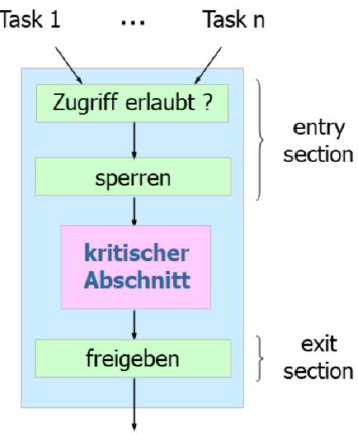
\includegraphics[width=500px]{img/kritischerAbschnittLsg.png}
	\captionof{figure}{Struktur der Lösung eines kritischen Abschnittes}
	\label{fig:Struktur der Lösung eines kritischen Abschnittes}
\end{Figure}

	\subsection{Anforderung an die Lösung}
\begin{enumeration}
	\item jeweils nur eine Aufgabe in ihren kritischen Abschnitt aufgenommen werden darf
	\item es werden keine Annahmen über relative Aufgabengeschwindigkeiten oder die Anzahl der Prozessoren getroffen
	\item ein Task, die in ihrem unkritischen Teil stehen bleibt, muss dies tun, ohne andere Aufgaben zu behindern
	\item ein Task, die Zugang zu einem kritischen Abschnitt erfordern, dürfen nicht auf unbestimmte Zeit verzögert werden
	\item kein Prozess befindet sich in einem kritischen Abschnitt: jede Aufgabe, die den Eintritt in die Krippenabteilung verlangt, muss ohne Verzögerung zugelassen werden
	\item ein Task darf nur für eine begrenzte Zeit innerhalb ihres kritischen Abschnitts bleiben
\end{enumeration}



\section{Sie können das Consumer/Producer und Readers/Writers Problem erklären und diskutieren}
	\subsection{Producer-Consumer Problem}
Es geht um die koordinierte Datenausgabe $\rightarrow$ Mehrere Producer-Tasks produzieren Ausgabedaten und ein Consumer-Task übernimmt die Daten und gibt sie aus
\begin{Figure}
\centering
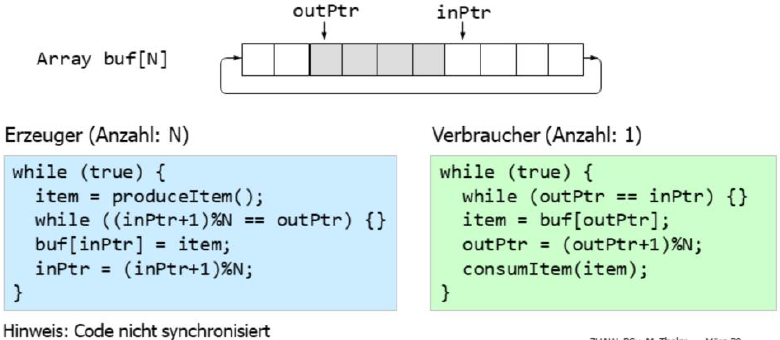
\includegraphics[width=500px]{img/gemRingBuffer.png}
	\captionof{figure}{Beispiel einer Lösung für das Producer-Consumer-Problem}
	\label{fig:Beispiel einer Lösung für das Producer-Consumer-Problem}
\end{Figure}

	\subsection{Readers-Writer-Problem}
Bei gemeinsamen Daten wird häufiger gelesen, als geschrieben (bspw. Datenbanken, Hash-Tabellen etc.). Dabei gibt es einen erweiterten kritischen Abschnitt.
\begin{itemize}
	\item mehrere Reader gleichzeitig im kritischen Abschnitt
	\item maximal ein Writer und kein Reader im kritischen Abschnitt
\end{itemize}
\begin{Figure}
\centering
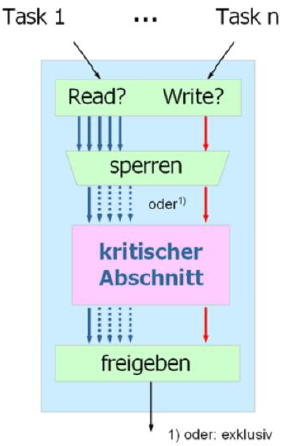
\includegraphics[width=500px]{img/RW-Problem.png}
	\captionof{figure}{Beispiel einer Lösung für das Reader-Writer-Problems}
	\label{fig:Beispiel einer Lösung für das Reader-Writer-Problems}
\end{Figure}

\section{Sie können Mechanismen für die Implementation von kritischen Abschnitten und zur Lösung von Synchronisations-Problemen aufzählen und erklären (Hardewareunterstützung für Synchronisationsmechanismen; Softwarelösungen; Semaphore, Monitore, Transactional Memory}
Dies kann mit unterschiedlichen Ansätzen erfolgen:
\begin{itemize}
	\item Reine Softwarelösungen $\rightarrow$ Software-Algorithmen, deren Korrektheit von keinen weiteren Bedingungen abhängt
	\item Hardwarelösungen $\rightarrow$ Unterstützung durch spezielle Maschineninstruktionen
	\item Lösungen mit Hilfe des Betriebssystems $\rightarrow$ Stellen dem Anwender Funktionen und Datenstrukturen zur Verfügung
	\item Lösungen zusammen mit Programmiersprchen $\rightarrow$ Monitore, z.B. Java
\end{itemize}

	\subsection{Softwarelösung}

		\subsubsection{Busy-wait}
Beim Busy-wait wartet der Task aktiv, d.h. er konsumiert Rechenzeit, bis der Scheduler einen Task-Switch durchführt $\rightarrow$ auch Spinlock genannt.
\begin{itemize}
	\item auf Uniprozessoren problematisch
	\item je nach Anwendung auf Mutlicore-Prozessoren sinnvoll
	\item gegenseitiger Ausschluss wird erreicht, aber die Tasks können nur abwechselnd den kritischen Abschnitt durchlaufen
	\item $\Rightarrow$ Der Task hinderst sich ausserhalb des kritischen Abschnitts selbst, den kritischen Abschnitt zweimal hintereinander zu betreten ($\rightarrow Widerspricht der Forderung 3$)
\end{itemize}
\begin{Figure}
\centering
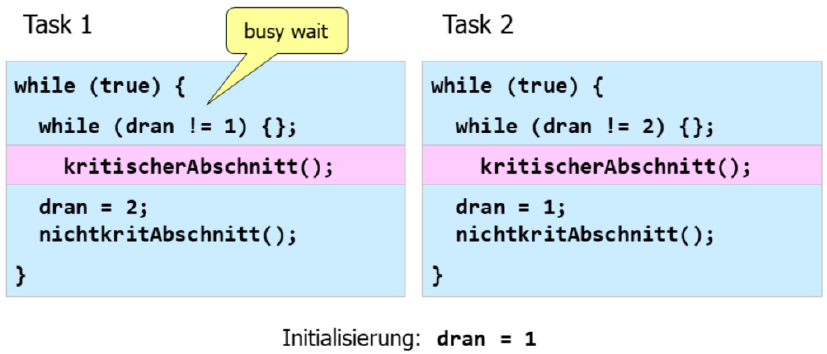
\includegraphics[width=500px]{img/busyWait.png}
	\captionof{figure}{Lösungsansatz mit Busy-Wait}
	\label{fig:Lösungsansatz mit Busy-Wait}
\end{Figure}

		\subsubsection{Peterson 1981}
\begin{itemize}
	\item sinnvoll bei unkritischem zeitlichen Ablauf
	\item ist nur für zwei Tasks geeignet
	\item busy-wait $\rightarrow$ Prozess wartet in Rechenschleife auf Freigabe des kritischen Abschnitts
	\item \textbf{Wichtig!} Funktioniert nicht auf modernen Multicore-Prozessoren
\end{itemize}
\begin{Figure}
\centering
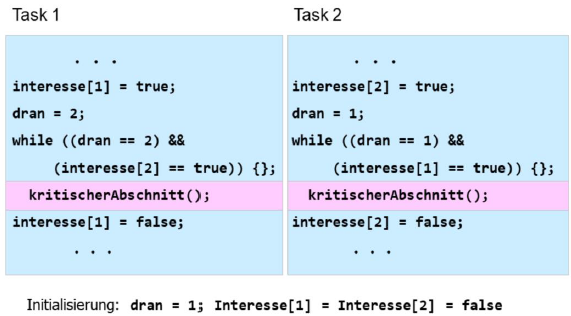
\includegraphics[width=500px]{img/Peterson1981.png}
	\captionof{figure}{Lösungsansatz mit Peterson 1981}
	\label{fig:Lösungsansatz mit Peterson 1981}
\end{Figure}

	\subsection{Hardwarelösungen}
verhindert, dass laufende Programme an beliebigen Stellen unterbrochen werden können. Dazu gibt es unterschiedliche Möglichkeiten:

\begin{itemize}
	\item Interrupt ausschalten
	\item atomare Intrusktionen für TAS (Test And Set) und CAS (Compare And Swap)
\end{itemize}
$\rightarrow$ man stösst auf ähnliche Probleme wie bei der Softwarelösungen $\Rightarrow$ Hardware ist nur eine Unterstützung keine Lösung

\textbf{To-Do: Müssen diese Variante noch weiter im Detail angeschaut werden?}


\chapter{Vorlesung 7 - Deadlocks}

\section{Sie können die Begriffe Deadlock, Lifelock und Starvation erklären und diskutieren}
	\subsection{Deadlock}
Beim Deadlock (zu Deutsch: Verklemmung) warten Tasks auf die gegenseitige Freigabe von Ressourcen $\Rightarrow$ Kein Task arbeitet weiter, es geht nicht mehr weiter
		\subsubsection{Voraussetzung}
\begin{enumerate}
	\item Mutual exclusion $\rightarrow$ mind. eine Ressource ist exklusiv reserviert
	\item Hold and wait $\rightarrow$ mind. ein Task hat eine Ressource exklusiv reserviert und wartet auf weitere Ressourcen
	\item No preemption $\rightarrow$ reservierte Ressourcen können dem Task nicht entzogen werden 
	\item Circular wait $\rightarrow$ geschlossene Kette von Tasks existiert, in der jeder Prozess mind. eine Ressource reserviert hat, die auch von einem Nachfolger in der Kette benötigtwird
\end{enumerate}
$\Rightarrow$ Es müssen alle Bedingungen gegeben sein, damit der Deadlock eintritt

	\subsection{Livelock}
Beim Livelock arbeitet der Task zwar weiter, jedoch ist die Arbeit nicht produktiv $\Rightarrow$ ungewollter busy-wait

	\subsection{Starvation}
Bei der Starvation (zu Deutsch: Verhungern) erhält der Prozess keinen Zugriff auf Ressourcen, dies kann beispielsweise bei einer unfairen Zuweisungspolicy unter anderem bei einem Stack (FILO-Prinzip) $\Rightarrow$ Abhilfe kann durch eine faire Policy geschaffen werden, bspw. FIFO


\section{Sie können die Möglichkeiten zur Verhinderung von Deadlocks aufzählen und diskutieren}
Dabei gibt es drei Möglichkeiten
\begin{itemize}
	\item Keine Deadlocks zulassen $\rightarrow$ entweder verhindern oder vermeiden
	\item Deadlocks zulassen $\rightarrow$ Wird gelöst wenn er eintritt
	\item Problem ignorieren $\rightarrow$ Annahme dass keine Deadlocks auftreten
\end{itemize}

\subsubsection{Verhindern} 
Mind. eine der vier Bedingungen darf nicht eintreten\\
$\Rightarrow$ ineffiziente Ressourcennutzung, serialisierte Verarbeitung\\

\subsubsection{Vermeiden} 
Ressourcen nicht zusprechen, wenn Deadlockgefahr besteht\\ 
$\Rightarrow$ Alles ausser Circular Wait zulassen\\
$\Rightarrow$ Ressourcenanforderung $\rightarrow$ überprüfen ob ein Deadlock eintreten könnte, evtl Task nicht starten\\
$\Rightarrow$ System in sicherem Zustand $\rightarrow$ Ressourcenzuweisung führt nicht zu Deadlock
\subsubsection{Erkennen} 
Deadlocks zulassen, bei Auftreten die Situation lösen oder das System muss periodisch auf Deadlocks untersucht werden\\
$\Rightarrow$ Betriebssystem überprüft ob ein Deadlock aufgetreten ist, falls ja Deadlock auflösen und lauffähigen Zustand wiederherstellen\\
$\Rightarrow$ Die Überprüfung erfolgt wenn ein Task auf Ressourcen warten muss, zu einem spezifischen INtervall oder wenn die CPU Auslastung unter einen bestimmten Wert sinkt\\

\textit{Recovery Strategies:}\\
\begin{enumerate}
	\item alle beteiligten Tasks stoppen $\rightarrow$ Meist verwendete Strategie
	\item alle beteilitgten Tasks auf Checkpoint zurücksetzen $\rightarrow$ Rollback-Mechanismus notwendig, Risiko dass Deadlock wieder auftritt
	\item beteilitgte Tasks der Reihe nach stoppen, bis Deadlock gelöst (bspw. wenigesten CPU, wenigsten Output, wenigsten alloziert, kleinste Prio, längste geschätzte Rechenzeitn) $\rightarrow$ Kriterium zur Wahl, nach jedem Stopp Detektionsalgorithmus neustarten
	\item beteiligten Tasks Ressourcen wegnehmen, bis Deadlock gelöst (bspw. wenigesten CPU, wenigsten Output, wenigsten alloziert, kleinste Prio, längste geschätzte Rechenzeitn) $\rightarrow$ Kriterium zur Wahl, Rollback zum Punkt vor Ressourcenallokation
\end{enumerate}

\section{Sie können Ressourcengrafen erklären, diskutieren und Ressourcengrafen für das Finden von Deadlocks einsetzen}
Ist ein gerichteter Graf und stellt die Ressourcenzuordnung dar.\\
$\Rightarrow$ Wenn kein Zyklus vorhanden ist, gibt es auch keinen Deadlock
$\Rightarrow$ Wenn ein Zyklus vorhanden ist, gibt es:
\begin{itemize}
	\item eine Instanz pro Ressource $\rightarrow$ Deadlock
	\item mehrere Instanzen pro Ressource $\rightarrow$ Deadlock möglich
\end{itemize}
	\subsection{Elemente eines Ressourcengrafs}
\textbf{Kreis:} stellt einen Task dar\\
\textbf{Rechtecke:} stellen die Ressourcen dar\\
\textbf{Punkte in Rechteck}: jede INstanz entspricht einem Punkt innerhalb des Rechtecks
\textbf{Pfeil von Ressource zu Task:} der Task hat Ressource alloziert\\
\textbf{Pfeil von Task zu Ressource:} der Task fordert Ressource an\\


\section{Sie können abschätzen, ob Deadlocks bzw. Starvation kritisch oder unkritisch sind}
%Todo
Wo steht das? :) 

\chapter{Vorlesung 8 - Internprozess-Kommunikation}

\section{Sie können den Begriff Interprozesskommunikation erklären und erläutern}
Prozesse arbeiten zusammen um gemeinsam eine Aufgabe zu lösen bzw. gemeinsame Ressourcen zu nutzen $\rightarrow$ Hierfür ist Datenaustausch notwendig\\
Gründe für die Zusammenarbeit:
\begin{itemize}
	\item Parallelverarbeitung $\rightarrow$ Leistungssteigerung, Benutzerfreundlichkeit
	\item vereinfachte Strukturierung von Anwendungen $\rightarrow$ mehrere kooperiende, aber kleine Prozesse
	\item Daten- und Informationsaustausch $\rightarrow$ einfacher Zugriff auf gemeinsame Daten
	\item Echtzeitsysteme $\rightarrow$ Aufgaben mit unters. Repetitionsrate
\end{itemize}

Es können zwei mögliche Lösungsszenarien eintreten (wird anhand eines Druckauftrages aufgezeigt):
\begin{enumerate}
	\item Synchronisation $\rightarrow$ Nur ein Prozess darf drucken, die anderen müssen warten
	\item IPC $\rightarrow$ es gibt einen Druckprozess, welcher die Daten entgegen nimmt und anschliessend ausdruckt, wobei die Prozesse selber nicht drucken dürfen, darf weiterarbeiten können
\end{enumerate}

\section{Sie können Message Passing erklären und disktutieren}
Hierbei geht es um den Austausch von Nachrichten innerhalb eines oder verteilten Systeme. Das Betriebssystem stellt die Zugriffsfunktion zur Verfügung und die Synchronisation wird durch diese zugriffsfunktion definiert.\\
Dabei ist der Anwender verantwortlich für das Verpacken der Daten in Nachrichten (bspw. Message Queues)
\begin{itemize}
	\item Sehr häufiges Verfahren $\rightarrow$ zwischen Prozessen auf einem Rechner, verteilten Systemen, wobei die Synchronisation implizit ist
	\item Grundfunktion \textit{send(dest, message)} und \textit{receive(src, message)} $\Rightarrow$ beide Funktionen können blockieren
	\item auch geeignet für reine Prozess-Synchronisation oder Implementation eines Mutex
\end{itemize}

\begin{Figure}
\centering
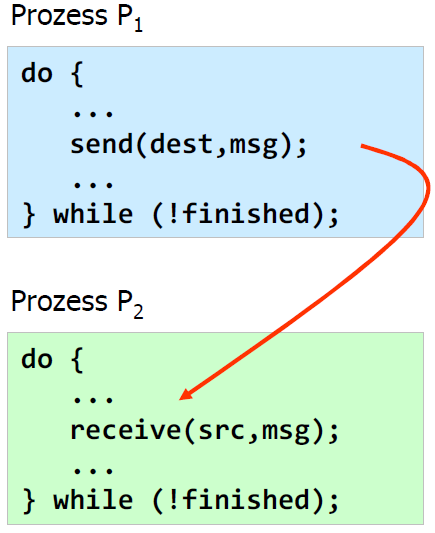
\includegraphics[width=500px]{img/MessagePassing.png}
	\captionof{figure}{Beispiel eines Message Passing}
	\label{fig:Beispiel eines Message Passing}
\end{Figure}

	\subsection{Verbindungsarten}
\textbf{Synchrone bzw. verbindungsorientierte} Kommunikation $\rightarrow$ beide Prozesse müssen der Verbindung zustimmen
\begin{Figure}
\centering
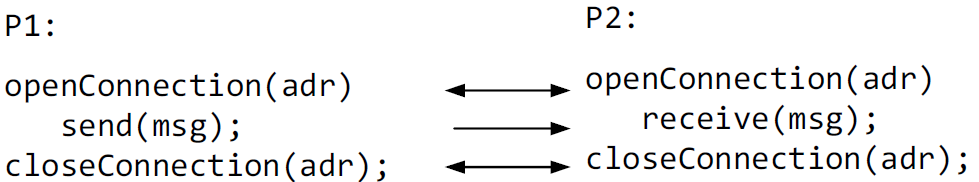
\includegraphics[width=500px]{img/MessagePassingSynchron.png}
	\captionof{figure}{Beispiel einer synchronen Message Passing}
	\label{fig:Beispiel einer synchronenMessage Passing}
\end{Figure}

\textbf{Asynchrone bzw. verbindungslose} Kommunikation $\rightarrow$ Sender schickt Nachricht einfach los. Allenfalls ist dabei eine Quittierung notwendig (Sache der Applikation)
\begin{Figure}
\centering
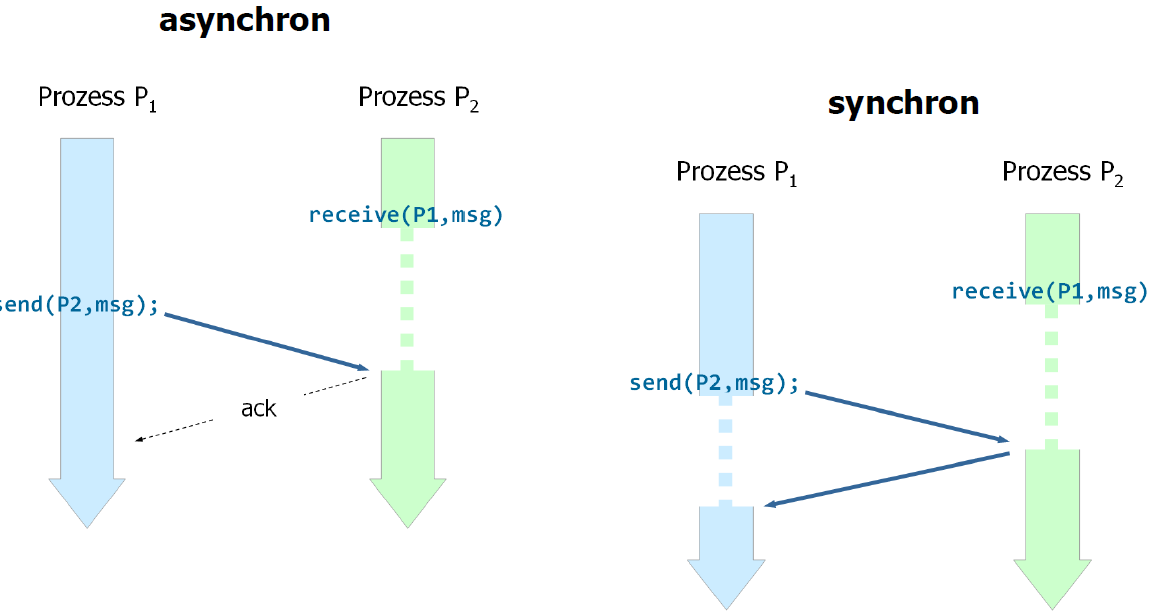
\includegraphics[width=500px]{img/MessagePassingSynchronAsynchron.png}
	\captionof{figure}{Unterschied synchron vs. asynchrones Message Passing}
	\label{fig:Unterschied synchron vs. asynchrones Message Passing}
\end{Figure}

	\subsection{Adressierung}
\textbf{direkte Adressierung}
\begin{itemize}
	\item Nachricht wird direkt in den Adressraum (Speicher) des Empfänger kooperiert
	\item Adressierung kann \textit{explizit} (Quelladresse wird beim Empfänger einer Nachricht angegeben) oder \textit{implizit} (Quelladresse kann nicht angegeben werden) erfolgen
	\item Sender und Empfänger sind eng gekoppelt
	\item Vorteil: geschützter Datenverkehr
\end{itemize}
\begin{Figure}
\centering
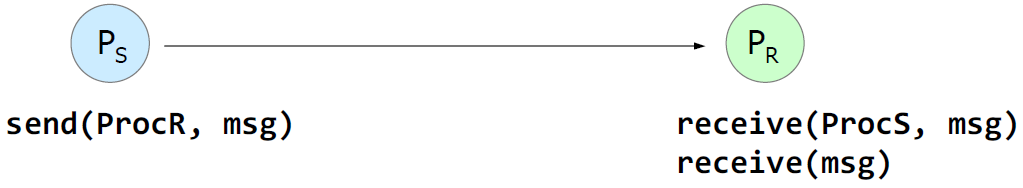
\includegraphics[width=500px]{img/MessagePassingDirekteAdressierung.png}
	\captionof{figure}{Beispiel einer direkten Adressierung}
	\label{fig:Beispiel einer direkten Adressierung}
\end{Figure}

\textbf{indirekte Adressierung}
\begin{itemize}
	\item Nachricht wird nicht direkt an den Empfänger gesendet
	\item Nachricht wird an eine Mailbox (bzw. Port) gesendet (Queue)
	\item Sender und Empfänger sind entkoppelt
	\item Vorteil: vers. Verbindungstopologien möglich
\end{itemize}
\begin{Figure}
\centering
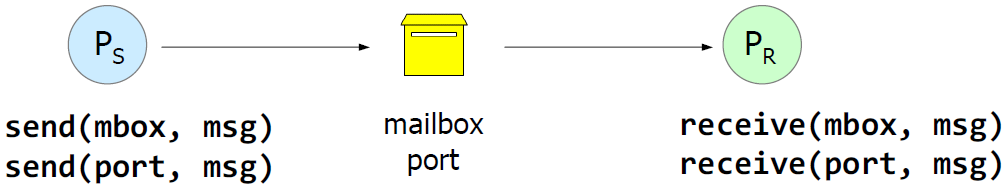
\includegraphics[width=500px]{img/MessagePassingIndirekteAdressierung.png}
	\captionof{figure}{Beispiel einer indirekten Adressierung}
	\label{fig:Beispiel einer indirekten Adressierung}
\end{Figure}
\begin{Figure}
\centering
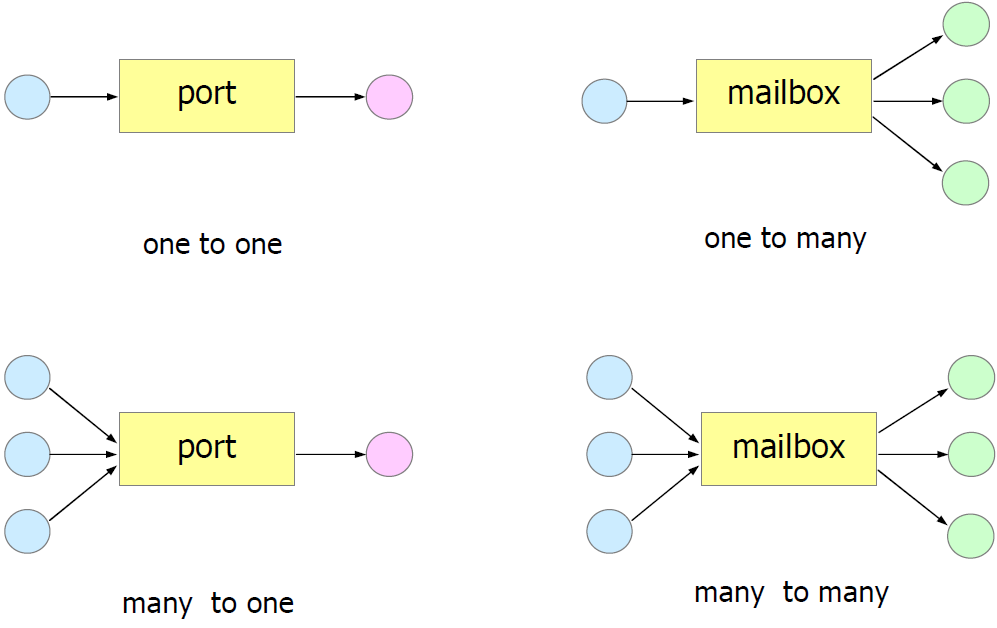
\includegraphics[width=500px]{img/MessagePassingIndirekteAdressierungVar.png}
	\captionof{figure}{Vers. Verbindungsvarianten}
	\label{fig:Vers. Verbindungsvarianten}
\end{Figure}

% Todo
\textbf{Mailbox V.06 S. 12 relevant?}
\textbf{Nachricht V.06 S. 13 relevant?}

\section{Sie können Shared Memory erklären und disktutieren}
Hierbei geht es um einen gemeinsamen Speicher, welches meist innerhalb eines gemeinsamen Systems ist. Das Betriebssystem stellt den gemeinsamen Speicherbereich zu Verfügung.\\
Dabei ist der Anwender verantwortlich für Datenstruktur und Synchronisation.\\
Der Bereich eines physikalischen Speichers wird in den (virtuellen) Addressraum der Prozesse abgebildet. Der physikalische Bereich kann an vers. Orte im virtuellen Adressraum eingebunden werden

\begin{Figure}
\centering
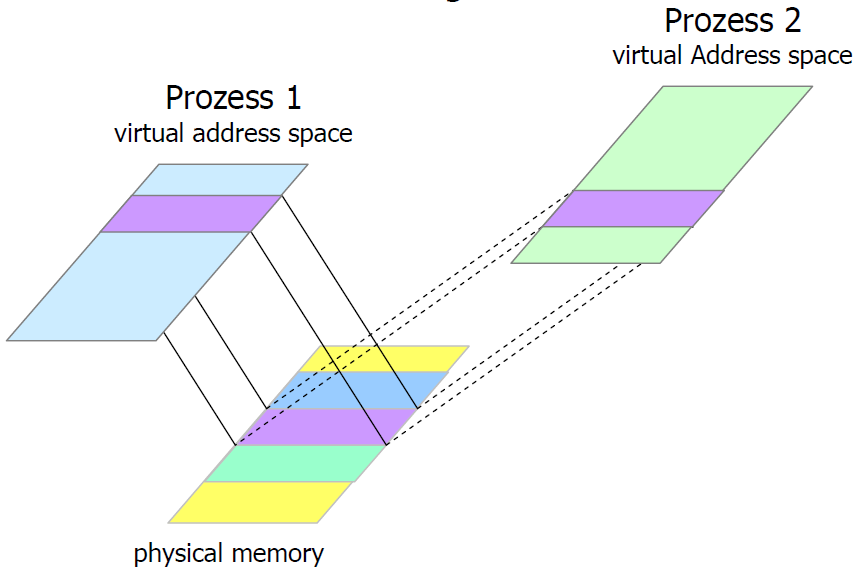
\includegraphics[width=500px]{img/sharedMemory.png}
	\captionof{figure}{Abbildung shared Memory}
	\label{fig:Abbildung shared Memory}
\end{Figure}

	\subsection{Shared Memory vs. Message Passing}
\textbf{Shared Memory}
\begin{itemize}
	\item Muss bei Betriebssystem angefordert werden
	\item keine implizite Synchronisation
	\item Zugriff sehr schnell: Speicherzugriff
	\item nur in Shared Memory Systemen verfügbar
\end{itemize}

\textbf{Message Passing}
\begin{itemize}
	\item Mailbox muss bei Betriebssystem angefordert werden
	\item implizite Synchronisation
	\item langsamer als Shared Memory
	\item auch in verteilten Umgebungen verfügbar
\end{itemize}

\section{Sie können Unix/Linux IPC Mechanismen aufzählen, erklären und disktutieren}
POSIX steht für \textit{Portable Operating System Interface}\\
\textbf{Interprozesskommunikation}
\begin{itemize}
	\item IPC Ressourcen
	\item Shared Memory
	\item Message Queues
	\item Signale
	\item Pipes
	\item Sockets
	\item Shared Files / Memory Mapped Files
\end{itemize}

%todo
\textbf{Code beispiel für die einzelnen Varianten}

\textbf{Synchronisation}
\begin{itemize}
	\item Semaphore
	\item Lock Files
\end{itemize}


\section{Sie können Implementationsaspekte anhand der Unix/Linux IPC Mechanisem erklären und disktutieren}

% Todo

\chapter{Vorlesung 9 - Memory Management, Virtual Memory}
Das Memory Management ist für die Speicherverwaltung im Betriebssystem zuständig, da sich der Programmierer und Anwender nicht um den Speicher kümmern will.\\
\textbf{Uniprocessing:} Ein Prozess und das OS stehen im Speicher\\
\textbf{Multiprogramming:} Mehere Prozesse und das OS stehen im Speicher; div. Verwaltungsprozesse; bessere CPU-Nutzung\\ 

Dazu gehören folgende Einheiten
\begin{itemize}
	\item Logical Organisation $\rightarrow$ logischer Adressraum, lineare Folge von Bytes (words) $\Rightarrow$ Was sieht der Anwender
	\item Physical Organisation $\rightarrow$ physikalische Realisierung (Cache-, Haupt-, Sekundärspeicher) $\Rightarrow$ Was sieht das Betriebssystem
	\item Protection $\rightarrow$ verhindern, dass sich Prozesse gegenseitig beeinflussen
	\item Sharing $\rightarrow$ gemeinsame Speicherbereiche zur Verfügung stellen
	\item Relocation $\rightarrow$ verschieben eines Prozesses an bel. Ort im Speicher
\end{itemize}


\section{Sie können die Begriffe logische und physikalische Adresse erklären und diskutieren}
\textbf{logische Adresse:} Ist eine Referenz auf Speicherplatz, unabhängig von Speicherorganisation\\
\textbf{physikalische Adresse:} Ist eine Referenz auf physikalischer Speicherplatz\\

Dabei erzeugt der Compiler Code mit relativen (logischen) Adressen
\begin{Figure}
\centering
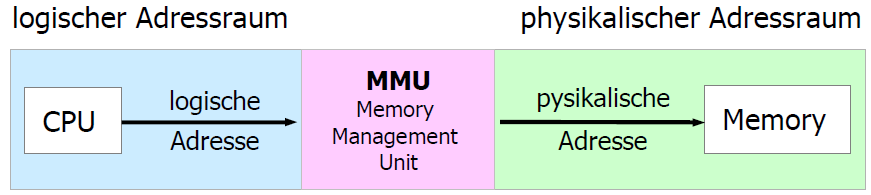
\includegraphics[width=500px]{img/logPhyMemMgmt.png}
	\captionof{figure}{Abbildung logische vs. physikalische Adressen}
	\label{fig:Abbildung logische vs. physikalische Adressen}
\end{Figure}

	\subcaption{Adressübersetzung}
\begin{itemize}
	\item CPU erzeugt logische bzw. virtuelle Adresse
	\item logische Adressen sind relativ, meist bezogen auf Adresse 0
	\item muss schnell und transparent sein $\rightarrow$ Hardewareunterstützung notwendig
\end{itemize}


\section{Sie können erklären, um was es beim Swapping geht}
Die Problematik ist, dass oft nicht alle Prozesse im Speicher Platz haben, aus diesem Grund lagert man einen Prozess vom Speicher auf Disk bzw. umgekehrt aus. Dies gilt auch für Teile eines Prozesses (virtual Memory).\\
$\rightarrow$ ausgelagerter Prozess ist suspendiert $\Rightarrow$ Heutzutage steht viel Speicher zur Verfügung, aus diesem Grund können auch ganze Prozesse im Speicher stehen.

\begin{Figure}
\centering
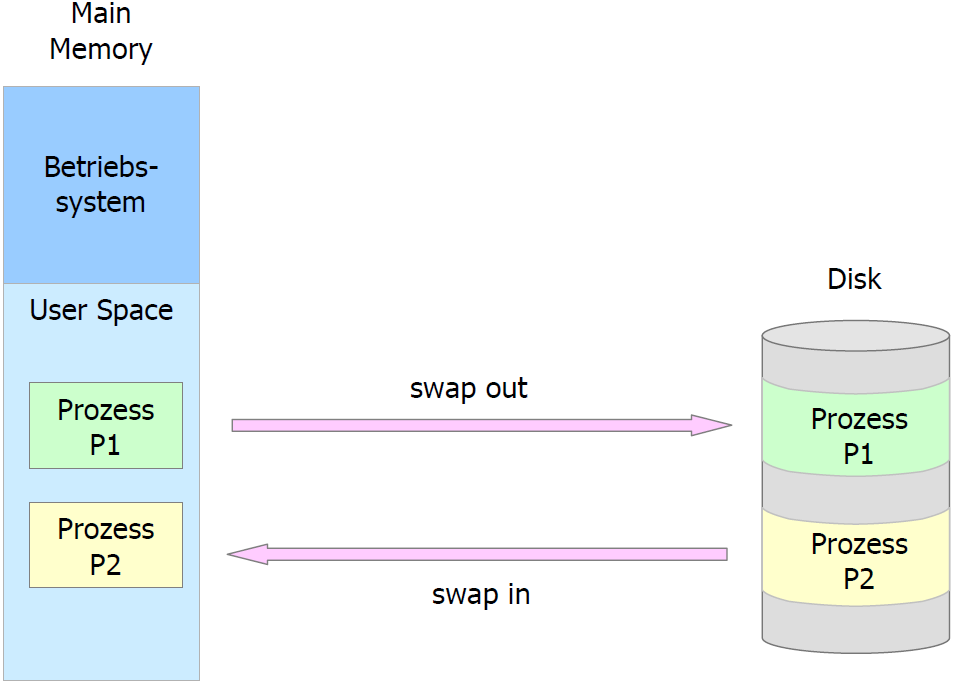
\includegraphics[width=500px]{img/Swapping.png}
	\captionof{figure}{Abbildung Swapping}
	\label{fig:Abbildung Swapping}
\end{Figure}



\section{Sie können die grundlegenden Verfahren des Memory Managements aufzählen und diskutieren}

	\subsection{Ansatz 1: einfaches Memory Management}
\begin{itemize}
	\item ganzer Prozess im Speicher
	\item traditioneller Ansatz
	\item einfaches Paging
	\item einfache Segmentation
	\item typische Anwendung: 'Kleine Systemen' $\rightarrow$ Embedded Systems, Real-Time Systeme
\end{itemize}

\textbf{Voraussetzung}
\begin{itemize}
	\item gesamter Prozess steht im Hauptspeicher
	\item unterstützt Multiprogramming
	\item für kleine / einfache Systeme
\end{itemize}

\textbf{mögliche Verfahren}
\begin{itemize}
	\item Addressraum zuteilen $\rightarrow$ fixed partitioning; dynamic partitioning; placement
	\item Addressraum aufteilen $\rightarrow$ paging; (Segmentation)
\end{itemize}
		
		\subsubsection{fixed partitioning}

\begin{itemize}
	\item Aufteilung des Hauptspeichers in mehrere nicht überlappende Partitionen $\rightarrow$ OS belegt feste Partition; vorgegebene Anzahl Prozesse im Speicher; BS kann Prozesse auslagern
	\item Gleich grosse Partitionen $\rightarrow$ jedes Programm, egal wie gross, belegt eine Partition; \textit{internal Fragmentation} wird eine nicht vollständig gefüllte Partition gennant; Nutzung des Hauptspeichers ist ineffizient
	\item verschieden grosse Partitionen $\rightarrow$ reduzieren, aber lösen nicht das Problem; V1: jede Partition eine Prozess-Queue (interne Fragmentierung minimieren, Queues bleiben leer); V2: für alle Partitionen eine Prozess Queue (besseres Multiprogramming, erhöht interne Fragmentierung) 
\end{itemize}

\begin{Figure}
\centering
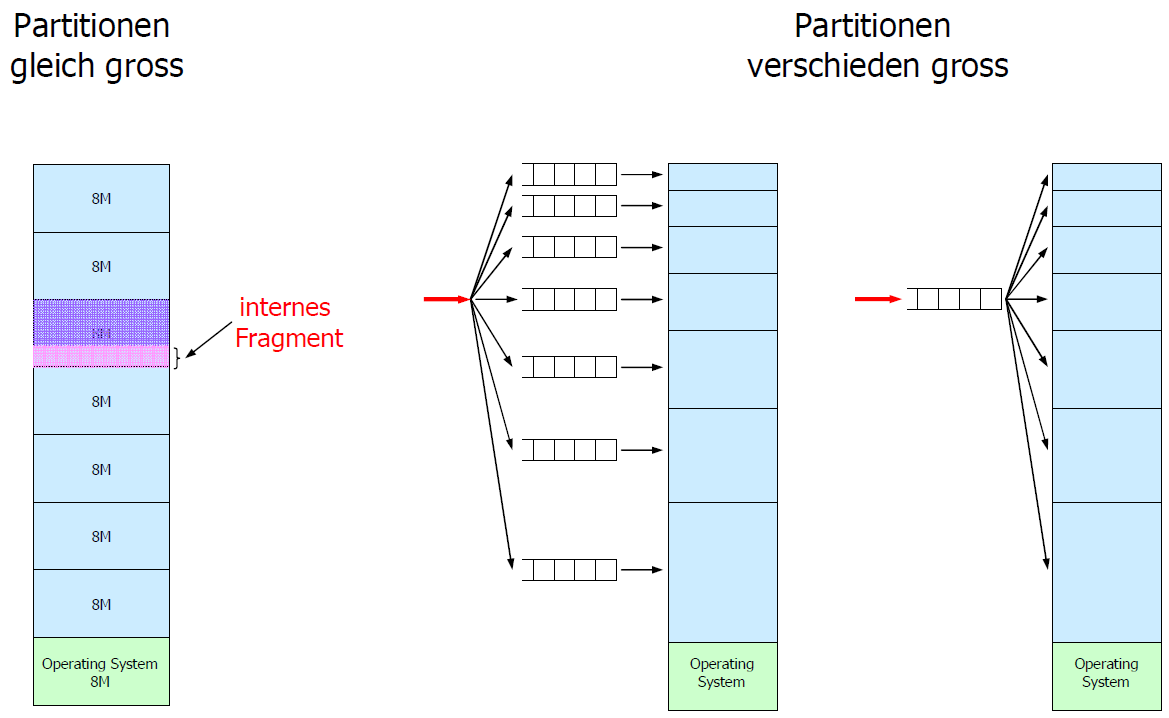
\includegraphics[width=500px]{img/FixedPartitioning.png}
	\captionof{figure}{Abbildung fixed partitioning}
	\label{fig:Abbildung fixed partitioning}
\end{Figure}

		\subsubsection{Dynamic Pratitioning}
\begin{itemize}
	\item Grösse und Anzahl der Partionen ist variabel $\rightarrow$ jedem Prozess so viel Speicher zuweisen wie er benötigt
	\item Problem: externe Fragmentierung, da Prozesse ausgelagert werden und nicht immer durch gleich grosse Prozesse ersetzt werden
	\item $\Rightarrow$ Compaction ist notwendig $\rightarrow$ Prozesse verschieben, bis Löcher geschlossen
\end{itemize}

Die Zuweisung kann durch verschiedene \textit{Placement Algorithmen} erfolgen
\begin{itemize}
	\item First Fit $\rightarrow$ einfachster und i.d.R. schnellster und bester Algorithmus $\Rightarrow$ Tendenziell weniger Fragementierung als bei Next-Fit
	\item Next Fit $\rightarrow$ alloziert oft freien Block am Schluss des Speichers, am Ende oft Blöcke am grössten $\Rightarrow$ Compaction öfters notwendig als bei First Fit
	\item Best Fit $\rightarrow$ sucht kleinsten, passender Block, minimiert externe Fragemente zum nächsten Block, entstehen schnell viele kleine Fragemente $\Rightarrow$ schlechtester Algorithmus (Compaction oft durchführen als bei First/Next Fit)
\end{itemize}

\begin{Figure}
\centering
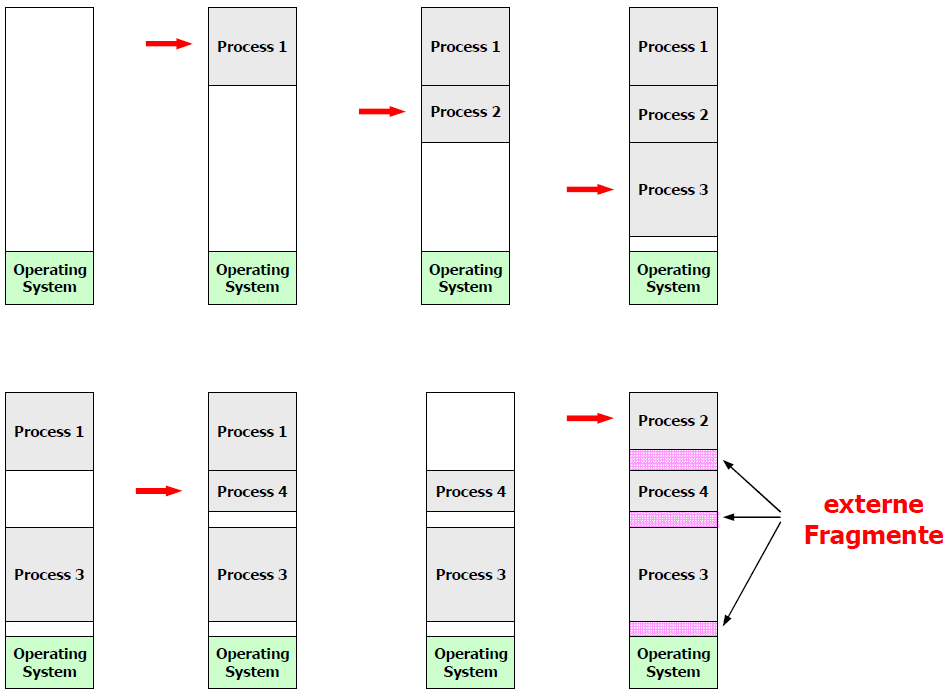
\includegraphics[width=500px]{img/DynamicPartitioning.png}
	\captionof{figure}{Abbildung dynamic partitioning}
	\label{fig:Abbildung dynamic partitioning}
\end{Figure}

		\subsubsection{Buddy System}
\begin{itemize}
	\item Kompromiss zwischen fixed und dynamic partitioning
	\item schneller Allokations- und Deallkokationsalgorithmus
	\item Unix/Linux verwendet modifizierte Buddy Systeme
\end{itemize}

\begin{Figure}
\centering
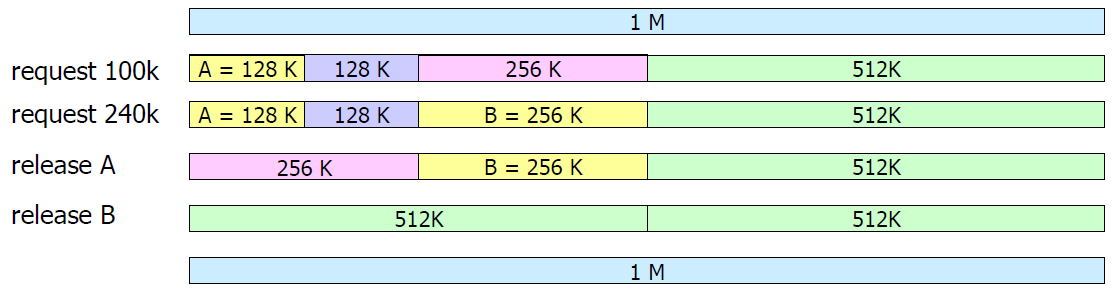
\includegraphics[width=500px]{img/BuddySysteme.png}
	\captionof{figure}{Abbildung Buddy System}
	\label{fig:Abbildung Buddy System}
\end{Figure}

\textbf{Algorithmus:}
\begin{itemize}
	\item es werden solange Blöcke halbiert, bis ein Block minimaler Grösse zur Verfügung steht
	\item Daten zum den freien Blöcken lassen sicht mit einem Binärbaum darstellen
	\item effiziente Algorithmen verfügbar (bspw. Stallings)
\end{itemize}

\begin{Figure}
\centering
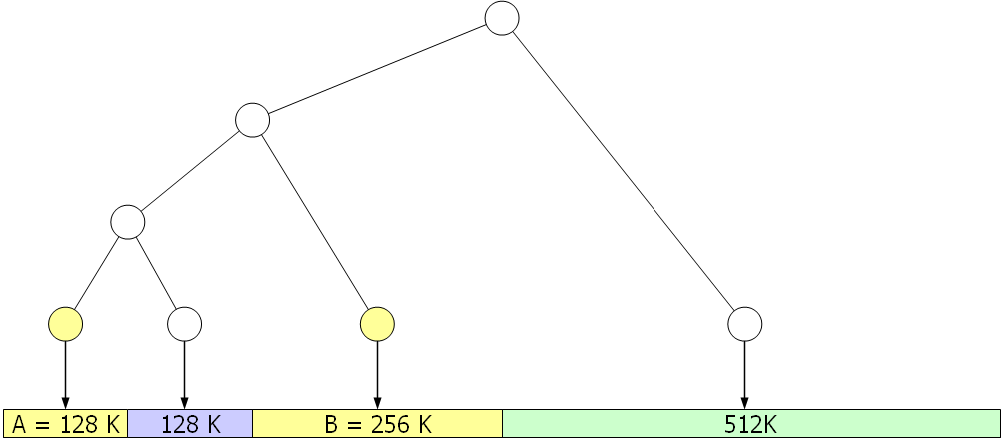
\includegraphics[width=500px]{img/BuddySystemeBinaryTree.png}
	\captionof{figure}{Abbildung eines Buddy System Binärbaums}
	\label{fig:Abbildung eines Buddy System Binärbaums}
\end{Figure}


	\subsection{Ansatz 2: Virutal Memory}
\begin{itemize}
	\item aktiver Teil des Prozesses im Speicher $\rightarrow$ Der Rest ist auf den Sekundärspeicher ausgelagert
	\item Paging
	\item virtualisiert den Speicher 
	\item Hard- und Softwareunterstützung notwendig
	\item typische Anwendung in 'grossen Systeme' $\rightarrow$ Workstation, Server, PCs
\end{itemize}

\begin{Figure}
\centering
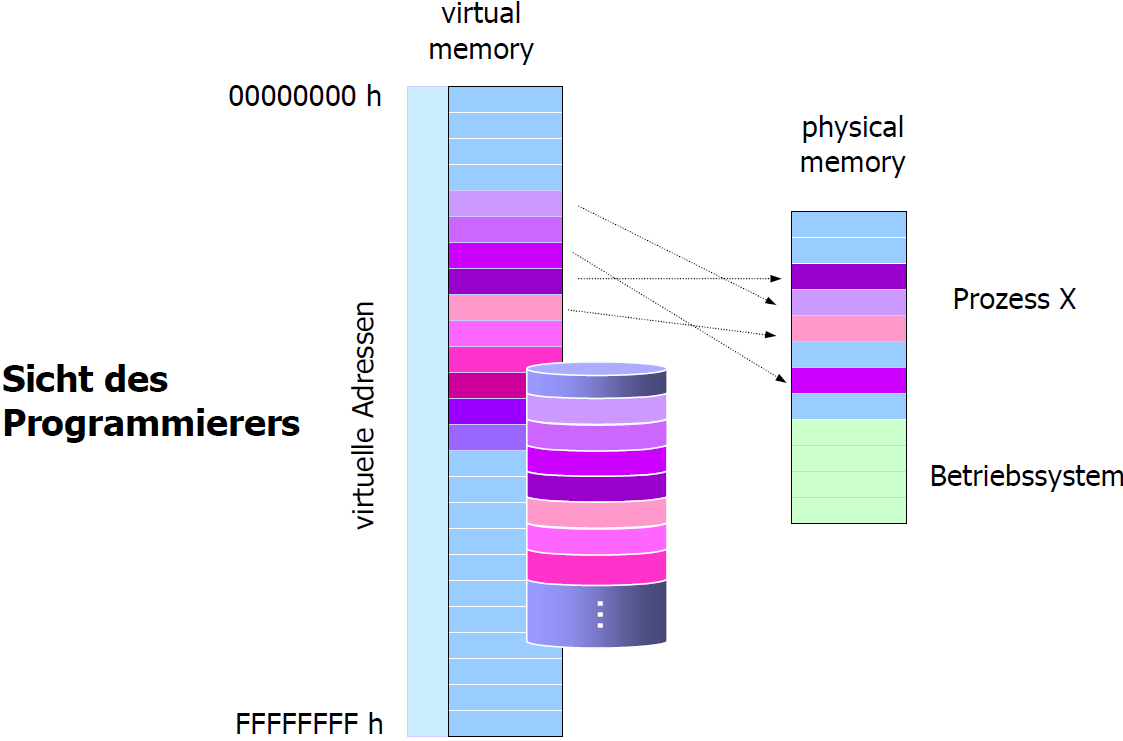
\includegraphics[width=500px]{img/VM.png}
	\captionof{figure}{Abbildung von virtual memory}
	\label{fig:Abbildung von virtual memory}
\end{Figure}

\begin{itemize}
	\item logischer resp. virtueller Adressraum in PAges aufgeteilt
	\item physikalischer Addressraum entsprechend in Frames aufteilt
	\item nur aktuell benötigte Pages im Hauptspeicher
	\item Rest der Pages als Image auf Disk
\end{itemize}

\textbf{Wie funktioniert VM:} Präozessor referenziert virtuelle Addresse\\
\textbf{Wieso funktioniert VM:} Virtual Memory basiert auf dem \textbf{Lokalitätsprinzip} $\rightarrow$ Speicherzugriffe liegen nahe beieinander, gleiche Instruktionen werden mehrmals ausgeführt\\
\textbf{Welche Pages stehen im Speicher:} BS muss bei Page-Fault intelligente Entscheidung treffen $\rightarrow$ OS versucht zu raten, welche Pages als nächste gebraucht werden

		\subsubsection{Page Table}
Das Realisieren von Page Table ist aufwendiger und benötigt zusätzliche Einträge

\begin{itemize}
	\item im virtuellen Memory kommen Page Tables zum Einsatz
	\item Realisierung aufwendiger, da zusätzliche Bits notwendig sind (siehe Abbildung)
	\item Adressübersetzung ist ähnlich wie beim Paging
	\item Page Tables werden gross
	\item Evtl. mehrere Speicherzugriffe notwendig $\rightarrow$ langsam
	\item Lösungen erfordern in der Regel Hardewareunterstützung
	\item Realisierung mittels Multilevel Organisation, Hashed Page Table oder Inverted Page Table
\end{itemize}

\begin{Figure}
\centering
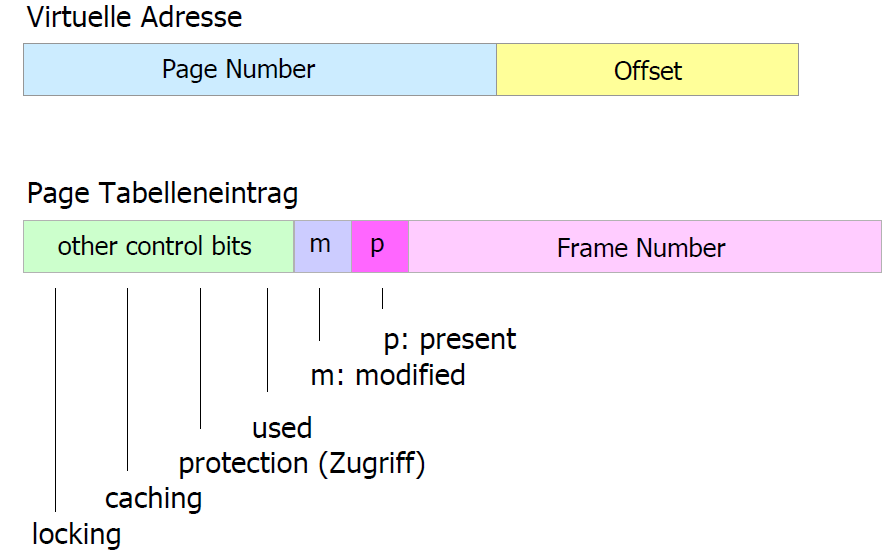
\includegraphics[width=500px]{img/PageTable.png}
	\captionof{figure}{Abbildung einer Page Table}
	\label{fig:Abbildung einer Page Table}
\end{Figure}

\textbf{Multilevel Organisation}\\
\textit{Beispiel gemäss Abbildung}
\begin{itemize}
	\item mehrere Page Directories (Verzeichnisse) und mehrere Page Tables
	\item 1. Stufe wählt Verzeichnisse
	\item 2. Stufe wählt Page Table
	\item minimale Anzahl von Tabellen $\rightarrow$ ein Page Directory und eine Page Tabelle
\end{itemize}

\begin{Figure}
\centering
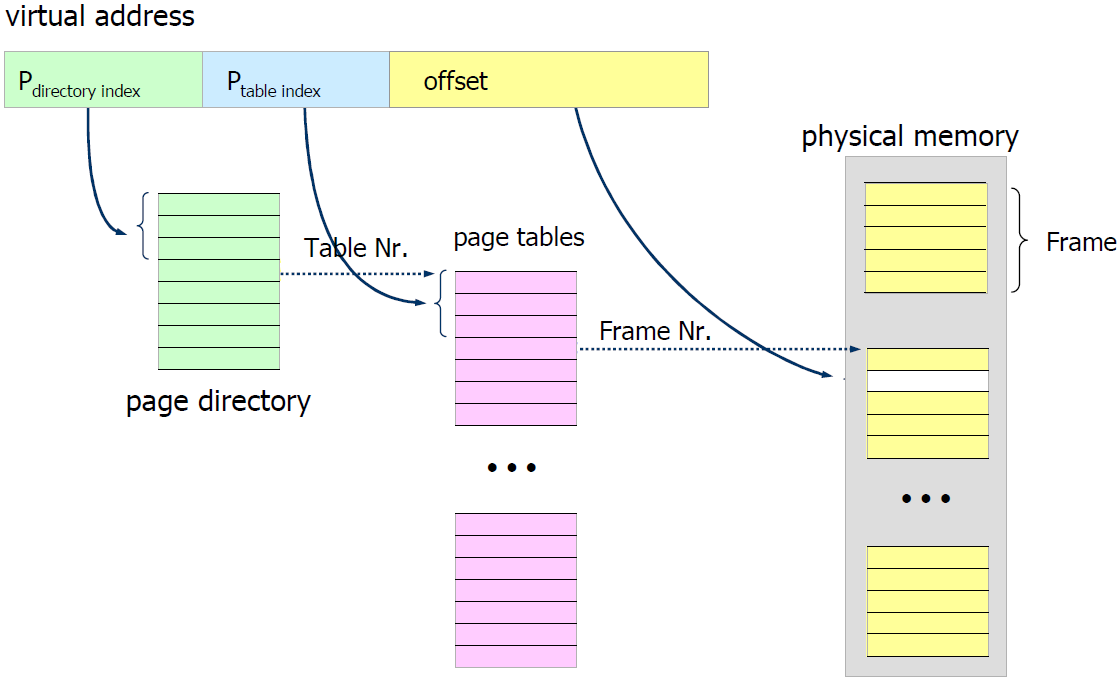
\includegraphics[width=500px]{img/MultilevelOrganisation.png}
	\captionof{figure}{Abbildung einer Multilevel Organisation}
	\label{fig:Abbildung einer Multilevel Organisation}
\end{Figure}

\textbf{Hashed Page Table}

\begin{itemize}
	\item Page Nummer wird als Hash-Wert verwendet
	\item verschiedene Page Nummern erzeugen gleicher Hash-Wert
	\item Hash-Tabelle: jeder Eintrag zeigt auf eine Liste mit den Einträgen
	\item Hash-Tabelle: jeder Listeeintrag enthält Page Nummer und entsprechende Frame Nummer
	\item bei Zugriff muss jeweils Page Nummer verglichen werden (gleicher Hash Wert)
	\item $\rightarrow$ zusätzlicher Aufwand, da Suche in Hash-Liste
	\item geeignet für invertierte Page Tabellen
	\item geeignet für Adressräume grösser 32 Bit
\end{itemize}

\begin{Figure}
\centering
\includegraphics[width=500px]{img/HashedPagedTable.png}
	\captionof{figure}{Abbildung einer Hashed Page Table}
	\label{fig:Abbildung einer Hashed Page Table}
\end{Figure}

\textbf{Inverted Page Table}
\begin{itemize}
	\item pro Frame gibt es einen Eintrag
	\item Nummern des Eintrags $j = $ Frame-Nummer
	\item gleiche Page von verschiedenen Prozessen in verschiedenen Frames abgelegt bzw. Prozess ID muss in Tabelle gespeichert werden
	\item Problem: ganze Tabelle muss nach Page-Nummer und PID abgesucht werden
	\item Problem: ineffizient, wenn vollständig in Software
	\item Im Einsatz bei PowerPC, UltraSPARC, ITHANIUM 
\end{itemize}

\begin{Figure}
\centering
\includegraphics[width=500px]{img/InvertedPagedTable.png}
	\captionof{figure}{Abbildung einer Inverted Page Table}
	\label{fig:Abbildung einer Inverted Page Table}
\end{Figure}

\section{Sie können Paging erklären und diskutieren}

\begin{itemize}
	\item logischer Addressraum der Prozesse wird in Pages aufgeteilt
	\item physikalischer Addressraum wird in Frames (Page Frames) aufgeteilt
	\item Pagegrösse = Framegrösse
\end{itemize}

Aktuelle Problematik:
\begin{itemize}
	\item Fixed Partitioning erzeugt interne Fragementierung
	\item Dynamic Partitioning erzeugt externe Fragementierung und erfordert Compaction
\end{itemize}

Mit Paging werden
\begin{itemize}
	\item Prozesse in Blöcke  gleicher Länge aufteilt $\rightarrow$ \textbf{Pages}
	\item Speicher in Blöcke gleicher Länge aufteteilt $\rightarrow$ \textbf{Frames}
	\item Die Zuweisung von Pages zu Frames ist beliebig $\rightarrow$ Prozess müssen nicht zusammenhängend im physikalischen Speicher stehen
\end{itemize}

	\subsection{Page Replacement}
Im Page Replacement werden folgende Fragen beantwortet:
\begin{itemize}
	\item welche Page ersetzen, wenn Speicher voll ist?
	\item welche Pages bzw. Frames kommen für Ersatz in Frage?
	\item wie viele Frames sollen einem Prozess zugewiesen werden?
\end{itemize}

$\rightarrow$ Wenn der Speicher voll: welche Page ersetzen?\\
Dabei kommen vier Replacement Policies ins Spiel: 
\begin{itemize}
	\item optimal
	\item least recently used
	\item fifo
	\item clock
\end{itemize}
Wobei das Bewertungskriterium die minimale Anzahl von Page Faults ist

		\subsubsection{Replacement Policy: optimal}
Ersetzt Page, die am spätesten referenziert wird $\rightarrow$ nicht implementierbar, aber beweisbar, dass minimale Anzahl Page Faults erreicht wurde\\
$\rightarrow$ gut geeignet für Vergleiche

\begin{Figure}
\centering
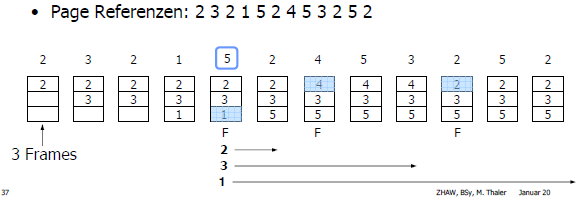
\includegraphics[width=500px]{img/ReplacementPolicyOptimal.png}
	\captionof{figure}{Abbildung der ReplacementPolicy: optimal}
	\label{fig:Abbildung der ReplacementPolicy: optimal}
\end{Figure}

		\subsubsection{Replacement Policy: least recently used}
Ersetzt die am längsten nicht referenzierte Page, welches fast so gut wie optimal funktioniert. Jedoch ist die Implementation aufwendig (TimeStamp oder UsageCounter notwendig)\\
$\rightarrow$ Funktioniert nach dem Lokalitätsprinzip, wird Wahrscheinlich nicht mehr referenziert

\begin{Figure}
\centering
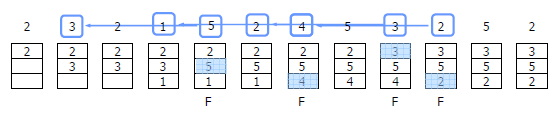
\includegraphics[width=500px]{img/ReplacementPolicyLRU.png}
	\captionof{figure}{Abbildung der ReplacementPolicy: least recently used}
	\label{fig:Abbildung der ReplacementPolicy: least recently used}
\end{Figure}

		\subsubsection{Replacement Policy: FIFO}
Pages Frames in zirkulärem Buffer angeordnet $\rightarrow$ älteste Page wird ersetzt, was sehr einfach zu implementieren ist - liefer jedoch schlechte Resultate\\
$\rightarrow$ Problematik, dass auch oft referenzierte Pages ausgelagert werden

\begin{Figure}
\centering
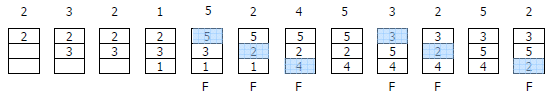
\includegraphics[width=500px]{img/ReplacementPolicyFIFO.png}
	\captionof{figure}{Abbildung der ReplacementPolicy: FIFO}
	\label{fig:Abbildung der ReplacementPolicy: FIFO}
\end{Figure}


		\subsubsection{Replacement Policy: Clock}
\begin{itemize}
	\item Anordnung in zirkulärem Buffer
	\item Ersetzt eine Page ausgehend von der Zeigerposition mit UseBit = 0 
	\item UseBit = 1 beim Laden
	\item schützt häufig referenzierte Seiten
	\item Kombination von LRU / FIFO
\end{itemize}

\begin{Figure}
\centering
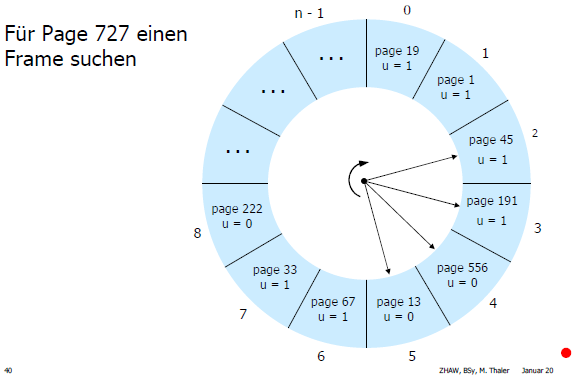
\includegraphics[width=500px]{img/ReplacementPolicyClock.png}
	\captionof{figure}{Abbildung der ReplacementPolicy: Clock}
	\label{fig:Abbildung der ReplacementPolicy: Clock}
\end{Figure}



\chapter{Vorlesung 10 - Input / Output Management}

Innerhalb eines PCs gibt es verschiedenste Peripheriebusse
\begin{itemize}
	\item AGP accelerated graphics port $\rightarrow$ stellt Grafik schnellen Zugriff auf Hauptspeicher zur Verfügung
	\item PCI peripheral component interconnect bus $\rightarrow$ universeller Peripherie Bus
	\item uvm
\end{itemize}

In der grossen Gerätevielfalt gibt es nur wenige Konzept wie Geräte an ein Computer angeschlossen werden und wie die Software die Hardware steuert.\\
Der Anschluss erfolgt über
\begin{itemize}
	\item Ports $\rightarrow$ ein Gerät, Datenstrom, z.B. serielle Schnittstelle
	\item Busse $\rightarrow$ mehrere Geräte, mehrere Drähte und ein Protokoll
\end{itemize}

\begin{Figure}
\centering
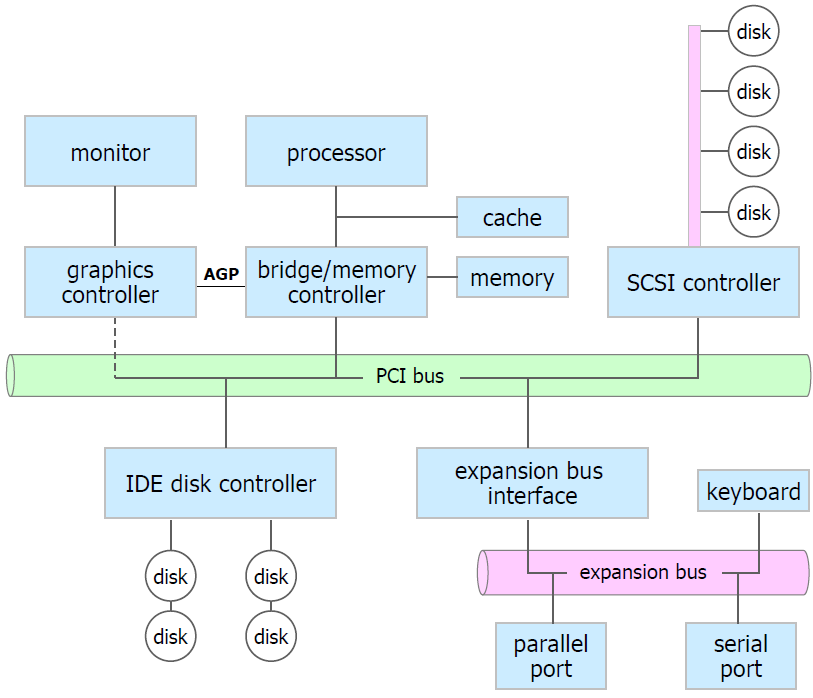
\includegraphics[width=500px]{img/PCArchitektur.png}
	\captionof{figure}{Abbildung eines PC Architektur}
	\label{fig:Abbildung eines PC Architektur}
\end{Figure}

\section{Sie können die grundlegende I/O-Architektur erklären und diskutieren}
\begin{itemize}
	\item Schichtenmodell
	\item wichtigste Komponente: Device Drivers $\rightarrow$ standardisierte Schnittstelle zum Kernel I/O-Subsystem und ist intern an Gerätedetails angepasst
	\item Keine vereinheitlichten Scnittstellen für Device Driver in Betriebssystemen $\rightarrow$ jedes Betriebssystem benötigt andere Treiber
	\item Logical I/O $\rightarrow$ Das Gerät wird als logische Resource betrachtet
	\item Device I/O $\rightarrow$ angeforderte Operationen in entsprechende Sequenzen von I/O Instruktionen umwandeln, Buffering
	\item Scheduling und Control $\rightarrow$ steuert den Ablauf der Interaktion zwischen Gerät und Software, Interrupt-Handling, IO Status etc.
	\item API $\rightarrow$ bei den meisten OS und Geräten
\end{itemize}

\begin{Figure}
\centering
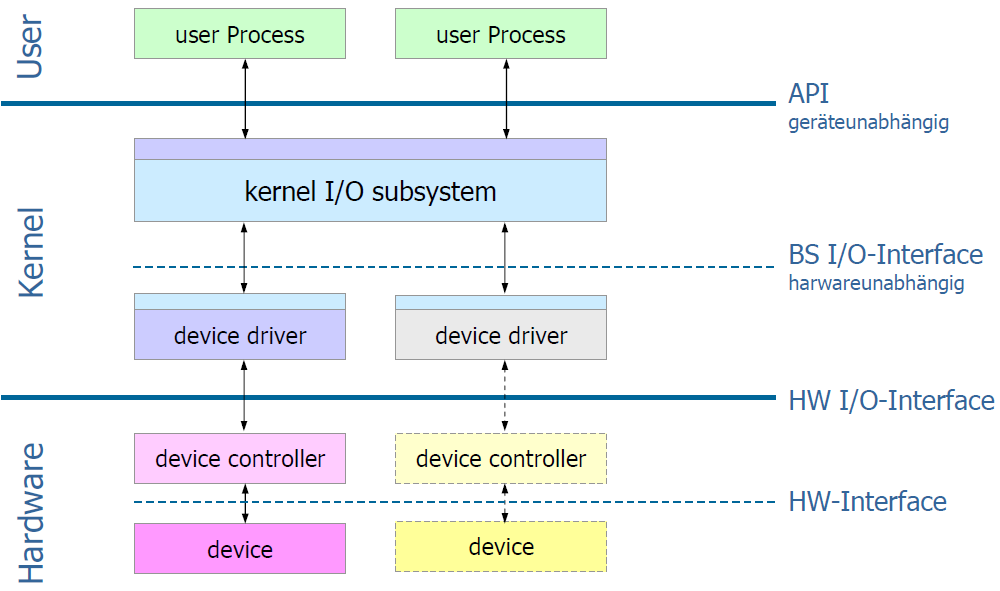
\includegraphics[width=500px]{img/IOArchitektur.png}
	\captionof{figure}{Abbildung der IO Architektur}
	\label{fig:Abbildung der IO Architektur}
\end{Figure}

	\subsection{Kernel I/O Subsystem}
\begin{itemize}
	\item I/O Scheduling $\rightarrow$ I/O-Anfragen von Anwendungen selten in optimaler Reihenfolge, OS ordnet Anfragen nach Optimierungskriterien (Performance, Fairness, Wartezeit)
	\item Buffering $\rightarrow$ Temporärerspeicher für Datenaustausch, da die Übertragungsgeschwindigkeit und Blockgrössen unterschiedlich sind
	\item Caching $\rightarrow$ hält Kopie der Daten für schnelleren Zugriff
	\item Spooling $\rightarrow$ Speicher mit Daten für Geräte die keine überlappenden Datenströme erlauben bspw. Drucker (oft durch Daemon)
	\item Reservation $\rightarrow$ Zugriffsreservation für nur exklusiv allozierbare Geräte
\end{itemize}


\section{Sie können die Konzepte des Linux Kernel I/O aufzeigen und diskutieren}

\begin{itemize}
	\item Gerätetypen $\rightarrow$ Block-, Stream- oder Netzwerkgeräte
	\item Schnittstelle zu Geräten: Filesystem $\rightarrow$ Geräte werden wie Files angesprochen
\end{itemize}

\begin{Figure}
\centering
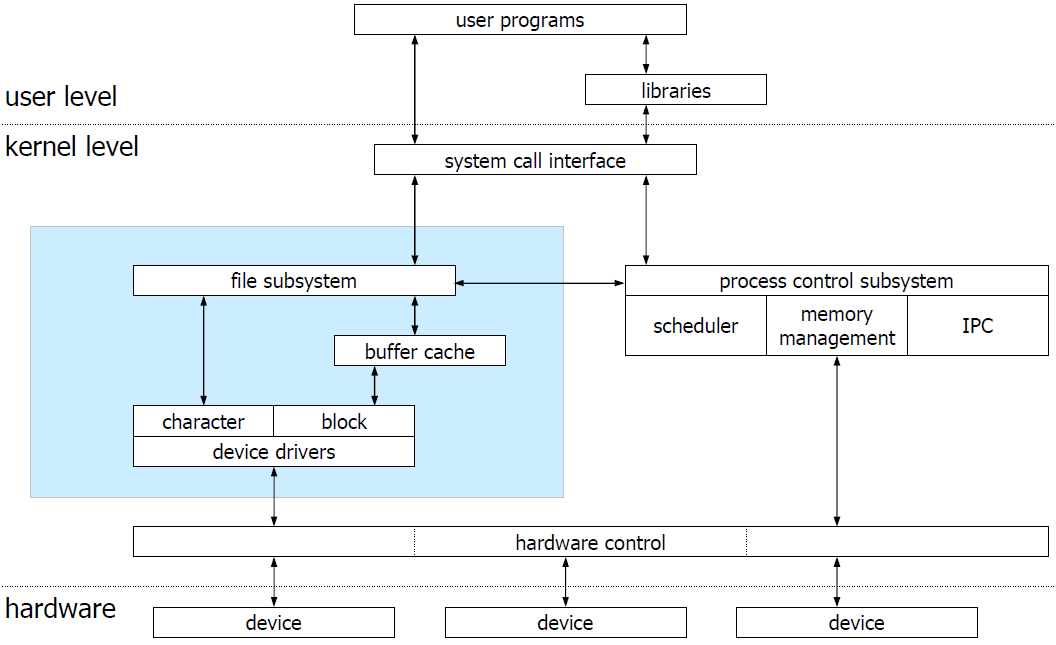
\includegraphics[width=500px]{img/LinuxIOArchitektur.png}
	\captionof{figure}{Abbildung der Linux IO Architektur}
	\label{fig:Abbildung der IO Linux Architektur}
\end{Figure}


\section{Sie können Charakteristiken von I/O Geräten aufzeigen  und diskutieren}

\begin{itemize}
	\item Stream $\rightarrow$ Datenübertragung Byte um Byte bspw. serielle Schnittstelle $\rightarrow$ charakteristisches Verhalten: spontan erzeugter Inputs
	\item Block $\rightarrow$ Datenübertragung als Block von Bytes (bspw. Disk) $\rightarrow$ charakteristisches Verhalten: random access
	\item Netzwerkgeräte erhalten Zugriff meist über Sockets
\end{itemize}


\begin{Figure}
\centering
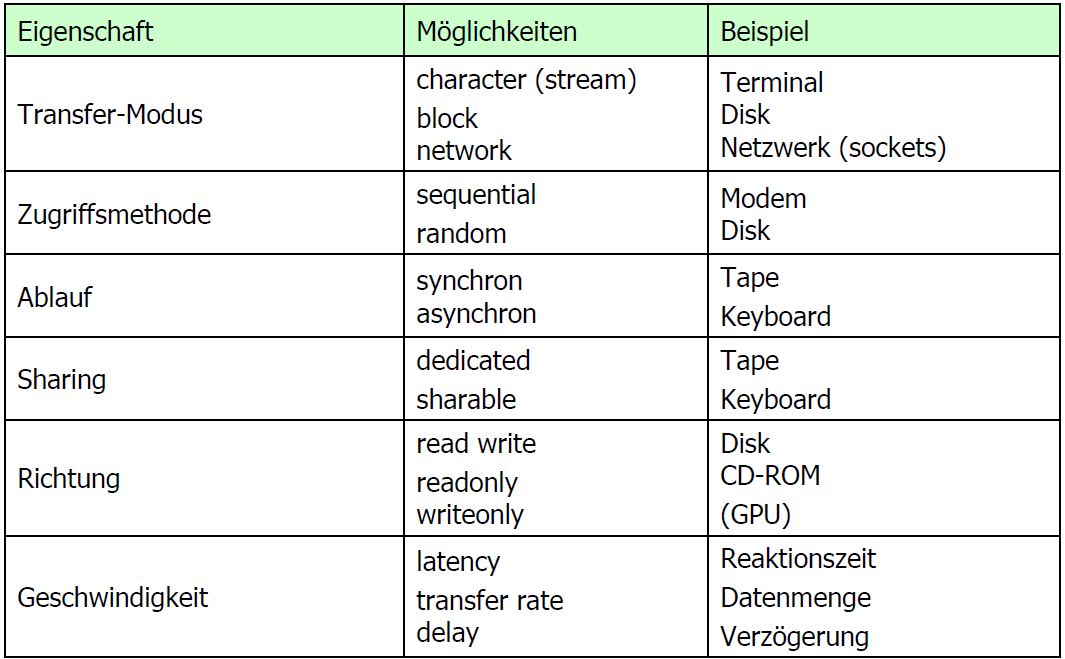
\includegraphics[width=500px]{img/IOCharakteristik.png}
	\captionof{figure}{Abbildung der IO Charakteristik}
	\label{fig:Abbildung der IO Charakteristik}
\end{Figure}

\begin{Figure}
\centering
\includegraphics[width=500px]{img/IOGeräteZugriff.png}
	\captionof{figure}{Abbildung der Linux Gerätezugriff}
	\label{fig:Abbildung der Linux Gerätezugriff}
\end{Figure}

\section{Sie können das Linux Modul/Treiber-System erklären}

\begin{itemize}
	\item geladenes Modul $\Rightarrow$ Teil des Kernels, realisiert Kernel-Code
	\item Treiber $\Rightarrow$ gehören zum Kernel, werden als Module realisiert
\end{itemize}

\begin{Figure}
\centering
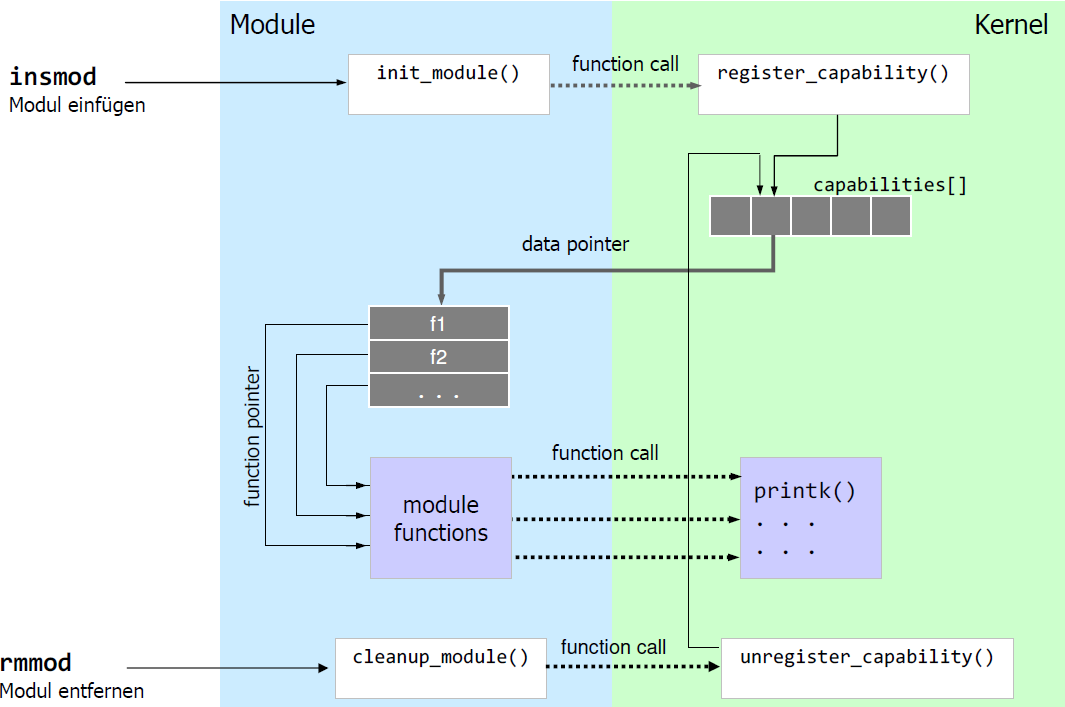
\includegraphics[width=500px]{img/LinuxTreiberModul.png}
	\captionof{figure}{Abbildung des Treiber vs. Modul in Linux}
	\label{fig:Abbildung des Treiber vs. Modul in Linux}
\end{Figure}

%ToDo: Ergänzen

\section{Sie können das Windows I/O System erklären}


\begin{Figure}
\centering
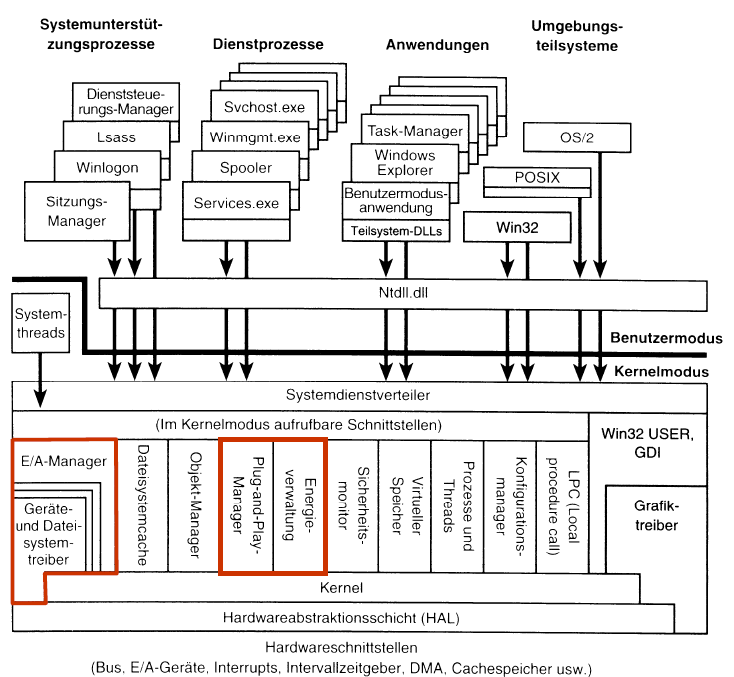
\includegraphics[width=500px]{img/WindowsNTArchitektur.png}
	\captionof{figure}{Abbildung des NT Architektur in Windows}
	\label{fig:Abbildung des NT Architektur in Windows}
\end{Figure}



\chapter{Vorlesung 11 - I/O Geräte}

\section{Sie können Problemstellungen bezüglich Disks aufzeigen und diskutieren}
Wie geht das Betriebssystem mit dem wichtigen Hardwarekomponente Disk um? 

	\subsection{Aufbau Disk}
\begin{itemize}
	\item mangetische Disk
	\item Sekundärspeicher
	\item sehr günstig
	\item in Platten organisiert
	\item Adressierung $\rightarrow$ 1D-Array von logischen Blocken, ein Block kleinste transferierbare Einheit
\end{itemize}

	\subsection{Diskzugriff}
\begin{enumerate}
	\item Anfrage durch Prozess (wartet bis Device bereit $t_w$; wartet auf Kanal $t_k$; Zugriff: $t_A$)
	\item Kopf auf Track positionieren $\rightarrow$ seek time
	\item warten bis Sektor unter Kopf $\rightarrow$ (rotational) latency
	\item Datentransfer
\end{enumerate}

\begin{Figure}
\centering
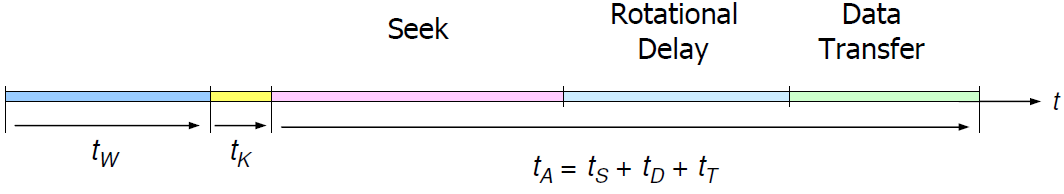
\includegraphics[width=500px]{img/Diskzugriff.png}
	\captionof{figure}{Abbildung des Diskzugriffs}
	\label{fig:Abbildung des Diskzugriffs}
\end{Figure}

%ToDo: Seite 7 - 15 ergänzen Slidesatz 08b


\section{Sie können Redundant Array of Independent Disks (RAIDs) erklären und disktutieren}
Grundidee: mit mehreren Disks einen zuverlässigen und schnellen Massenspeicher realisieren $\rightarrow$ Ausfall einer Disk darf nicht zum Systemausfall führen

\begin{itemize}
	\item verbessert Ausfallsicherheit des Massenspeichers
	\item mit Hot Spares: Reparaturzeit nahezu Null
	\item schützt nicht vor Viren, Löschen, Softwarefehler etc.
	\item Stromversorgung, Kabel etc. beeinflusst Verfügbarkeit
	\item muss an Anwendun angepasst sein
	\item Leseleistung $\geq$ Schreibleistung
\end{itemize}

\begin{Figure}
\centering
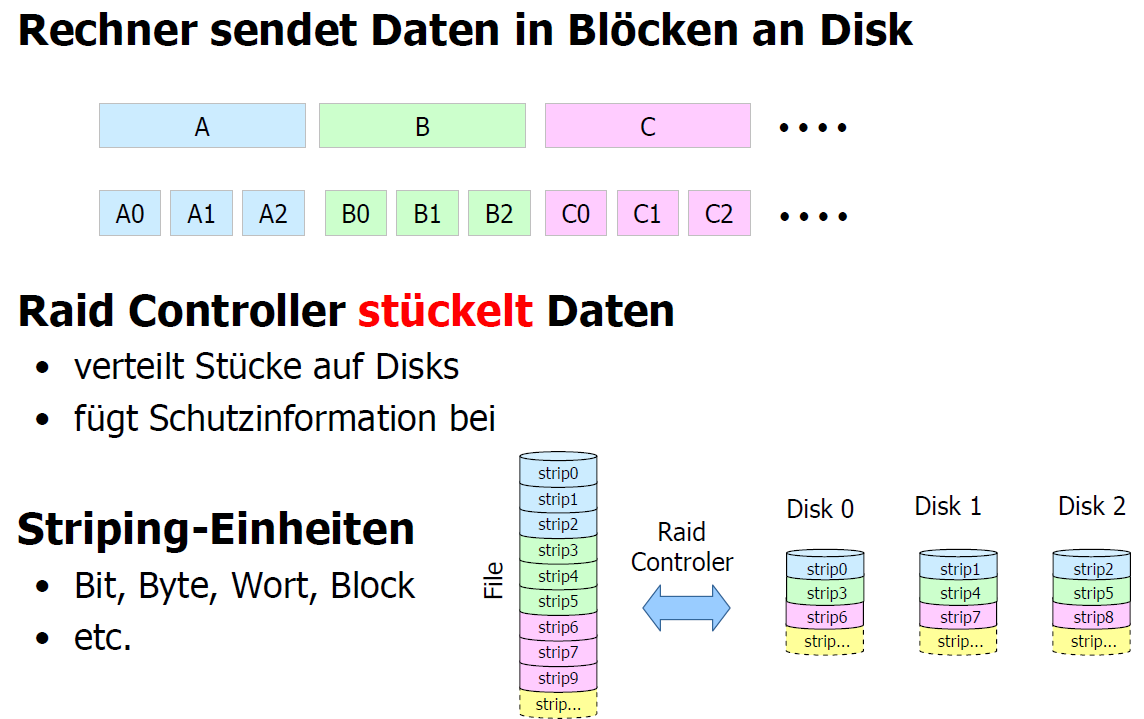
\includegraphics[width=500px]{img/RAIDPrinzip.png}
	\captionof{figure}{Abbildung des Grundprinzipes von RAID}
	\label{fig:Abbildung des Grundprinzipes von RAID}
\end{Figure}

\begin{Figure}
\centering
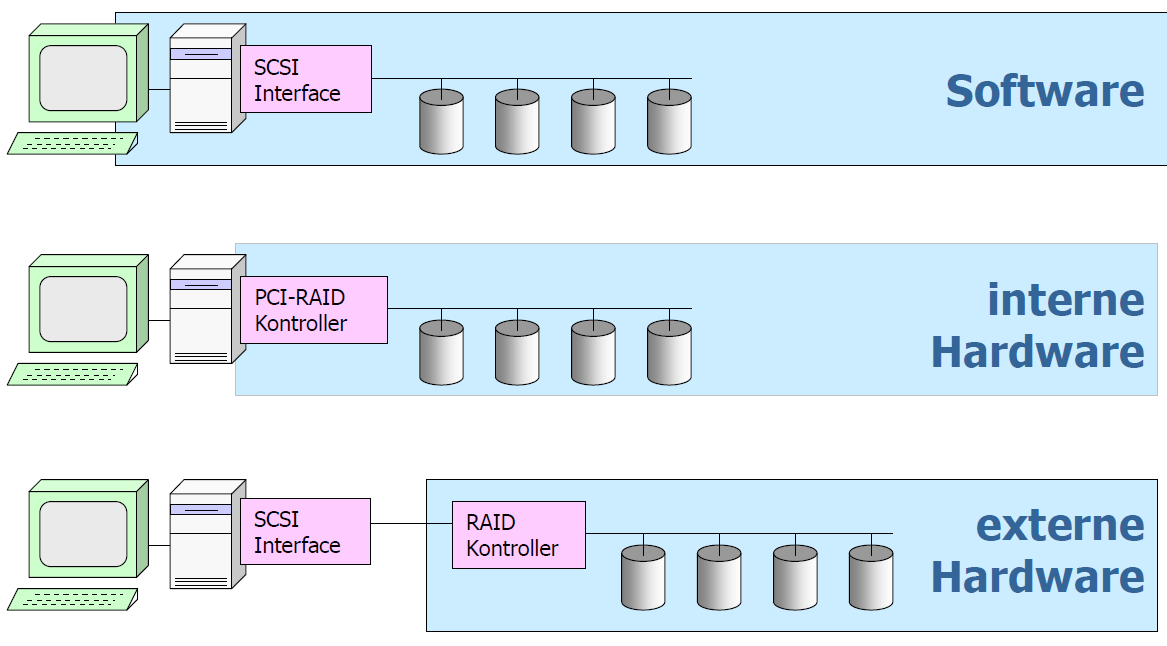
\includegraphics[width=500px]{img/RAIDFormen.png}
	\captionof{figure}{Abbildung Realisierungsformen von RAID}
	\label{fig:Abbildung Realisierungsformen von RAID}
\end{Figure}


\chapter{Vorlesung 12 - Filesystem}

\section{Sie können den Begriff File erklären und diskutieren}

\section{Sie können Anforderungen an das File System aufzählen und diskutieren}

\section{Sie können Operationenauf Files erklären und diskutieren}

\section{Sie können den File Zugriff erklären und diskutieren}

\section{Sie können die File System Architektur aufzeigen und erklären}

\section{Sie können File Allocation und Free Space Management erklären und diskutieren}

\section{Sie können File Management erklären und diskutieren}

\section{Sie können das Unix File System erklären und diskutieren, Filegrössen bestimmen}

\section{Sie können das Windows File System erklären und diskutieren}

\end{document}